\documentclass[12pt,lot,lof]{puthesis}
\usepackage{amsfonts}
\usepackage{amssymb}
\usepackage{amsmath}
\usepackage{amsthm}
\usepackage{latexsym}
\usepackage{graphicx}
%\usepackage[colorlinks=true, allcolors=blue]{hyperref}
%\usepackage{setspace}
\usepackage[square, numbers]{natbib} % for nice bibliography
\bibliographystyle{unsrtnat}

% \usepackage[backend=biber,style=numeric,sorting=none]{biblatex}


\title{The}
\submitted{May 2024}  %graduation date
\author{Ka Yu Stephanie Kwan}
\dedication{Placeholder dedication}
\adviser{Isobel Ojalvo}
\abstract{
Open questions in particle physics may be addressed by the existence of an extended Higgs sectorm beyond the Higgs boson with mass 125\GeV discovered in 2012 at the Large Hadron Collider (LHC) by the CMS and ATLAS experiments. Many properties of a potential extended Higgs sector remain unconstrained by current measurements, making direct searches of exotic Higgs decays a powerful probe of new physics. In extensions of the Standard Model of particle physics, such as Two Higgs Doublet Models extended with a singlet scalar (2HDM+S), the decay of the 125\GeV Higgs boson into light neutral scalar particles is allowed. We present a search at CMS for exotic decays of a Higgs boson with mass 125\GeV to two light neutral scalars, which respectively decay to two bottom quarks and two tau leptons (denoted $h\rightarrow aa \rightarrow bb\tau\tau$). This analysis is combined with a different search where the light scalars decay to two bottom quarks and two muons. Results are interpreted in various 2HDM+S scenarios. In Two Real Singlet Models (TRSMs), the 125\GeV Higgs boson can decay to two light neutral scalars with unequal mass, denoted $h \rightarrow a_1 a_2$ where $m_{a_1} \neq m_{a_2}$. This scenario has not been searched for to date at the CMS experiment. We present ongoing work on a search for $h\rightarrow a_1 a_2$, where the $a_2$ decays into two $a_1$, resulting in four bottom quarks and two tau leptons in the final state, in the $\mu\tau_{h}$ channel of the $\tau\tau$ decay. 
}

\acknowledgements{
Placeholder acknowledgements.
}

\begin{document}


\chapter{Introduction}
The Standard Model is the current prevailing theoretical framework that encompasses all known elementary particles to date and describes their interactions, yet falls short of describing open problems in physics. Here, we introduce the Standard Model (Section \ref{section:SM-history}) and provide a mathematical motivation of the SM a gauge theory (Section \ref{section:SM-as-gauge-theory}). We introduce the Higgs mechanism (Section \ref{section:Higgs-mechanism}), and outline two groups of theoretical extensions to the Standard Model that feature extended Higgs sectors (Sections \ref{section:theory-2HDM} and \ref{section:theory-TRSM}).

\section{History of the Standard Model}
\label{section:SM-history}
The building blocks of our modern-day understanding of particle physics were established over the course of decades by experimental discoveries and theoretical advances, culminating in the development of a theoretical framework known as the Standard Model (SM). In the 1880s, the electron was the first subatomic particle to be identified, through measurements of particles produced by ionizing gas. By the 1930s, atoms were known to consist mostly of empty space, with protons and neutrons concentrated at the center and orbited by electrons. Spurred by advances in particle accelerator technology, the experimental discoveries of the positron, the muon, and the pion, painted an increasingly complicated picture of particle physics that could not be described solely with atomic physics \cite{frampton_journeys_2001}.


In the absence of a theoretical framework describing these particles, in the 1960s and 1970s physicists and mathematicians developed the Standard Model to describe and encompass these fundamental particles and the forces that govern their interactions. The particle content of the Standard Model is shown in Fig. \ref{fig:intro-standard-model}: they are grouped into fermions, which comprise all known matter, and bosons, which mediate the interactions between particles.

\begin{figure}[ht]
    \centering
    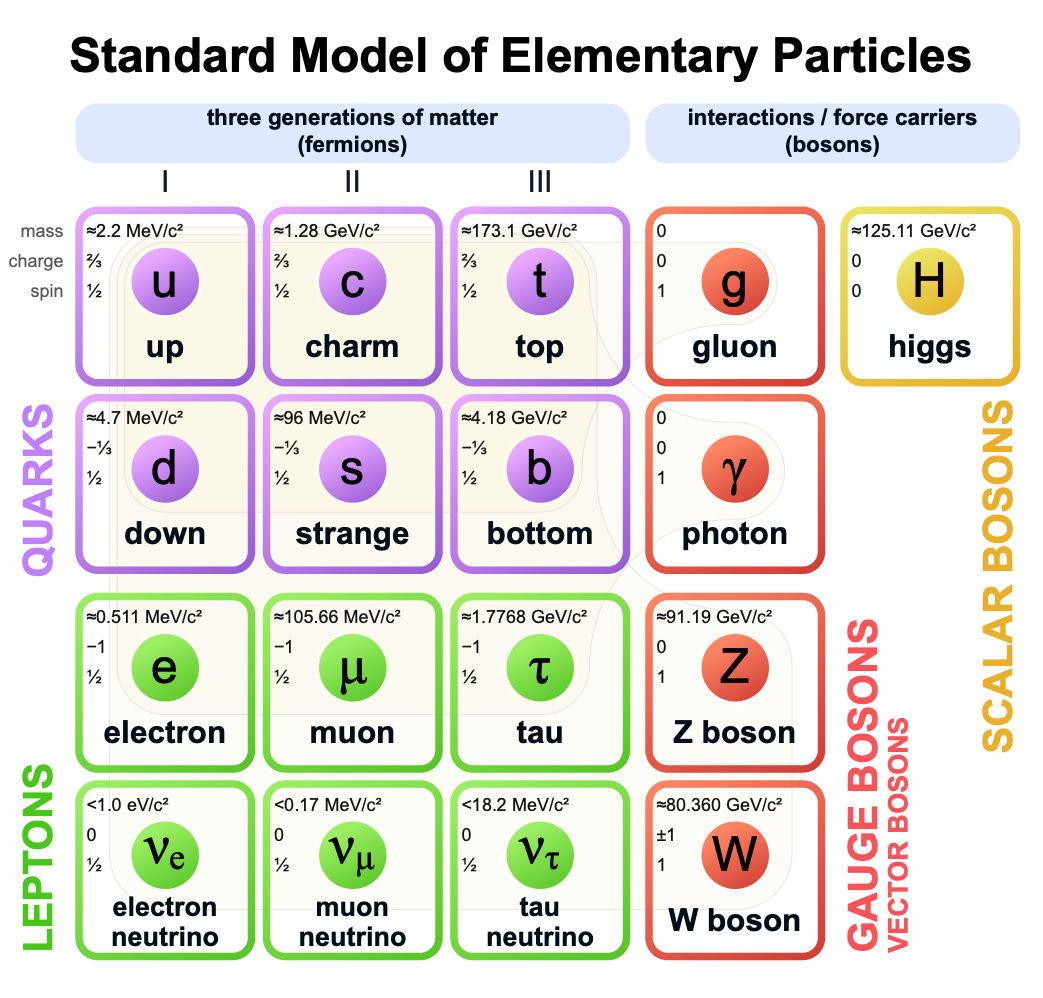
\includegraphics[width=8cm]{figures/ch-1-introduction/Standard_Model_of_Elementary_Particles.png}
    \caption{Table of Standard Model particles showing the grouping of the fermions into three generations of matter and the bosons, responsible for carrying the three fundamental forces in the Standard Model. The masses, charges, and spins of the particles are shown. The antimatter counterparts of the fermions are not shown. The possible interactions between the fermions and gauge bosons are highlighted.}
    \label{fig:intro-standard-model}
\end{figure}


Fermions consist of quarks and leptons, and are grouped into three generations. For example, the electron belongs to the first generation of leptons. The second and third generation counterparts of the electron are the muon and the tau lepton, and are over 200 and 30,000 times heavier than the electron respectively. Bosons are force carriers; the interaction of fermions with bosons corresponds to fundamental forces. The Standard Model describes the electromagnetic force, the strong nuclear force, and the weak nuclear force.


\section{The Standard Model as a gauge theory}
\label{section:SM-as-gauge-theory}

\subsection{Gauge invariance}
Gauge theories of elementary particle interactions originate from a freedom of choice in the mathematical description of particle fields which has no effect on the particles' physical states \cite{Tully+2012}. The existence and form of the particles' interactions, can be deduced from the existence of physically indeterminate, gaugable quantities.

An example of this gauge invariance is classical physics is the electromagnetic interaction, where the fundamental field is the four-vector potential $A^\mu$ \cite{Tully+2012}. The physical electromagnetic fields and Maxwell's equations arise from the elements of the tensor $F_{\mu\nu}(x) = \partial_\mu A_\nu (x) - \partial_\nu A_\mu (x)$. Any two choices of $A^\mu$ that are related by a transformation of the form

\begin{equation}
    A_\mu \rightarrow A_\mu + \partial_\mu \alpha
    \label{eqn:gauge_symmetry}
\end{equation} for any real, differentiable function $\alpha(x)$, describe the same physical configuration, and has no effect on Maxwell's equations. This ``redundancy'' in the choice of gauge in Eqn. \ref{eqn:gauge_symmetry} is called a gauge symmetry.

One important consequence of gauge symmetry comes from the application of Noether's theorem, which states that for every global transformation under which the Lagrangian density is invariant, there exists a conserved quantity. If $\mathcal{L}(\Psi(x), \partial_\mu \Psi(x))$ is invariant under the transformation of the wave function $\Psi(x) \rightarrow \Psi'(x)$, where $\Psi'(x) = \Psi(x) + \delta \Psi(x)$, then there exists a conserved current 
\begin{equation}
    \partial_\mu \left( \frac{\partial\mathcal{L}(x)}{\partial(\partial_\mu \Psi(x))} \delta \Psi(x)  \right) = 0
\end{equation}
In classical mechanics, the conservation of linear momentum, angular momentum, and energy follows from translational invariance, rotational variance, and invariance under translations in time \cite{Tully+2012}. Likewise, charge conservation can be shown to arise from the invariance of the Dirac Lagrangian density $\mathcal{L}_{\text{Dirac}} = \bar{\Psi} (i\gamma^\mu \partial_\mu -m)\Psi$ under the particle wavefunction's phase transformation, $\Psi'(x) = \exp(ie\chi) \Psi(x)$. Thus Noether's theorem establishes a correspondence between a gauge symmetry and a conserved internal property (e.g. charge or momentum).

\subsection{Local gauge symmetries}
Interactions between particles arise if we modify the wave function with a phase transformation $\Psi'(x) = \exp(i e \chi) \Psi(x)$, and allow the phase $\chi$ to be a function of spacetime \cite{Tully+2012}. A wave function of the form
\begin{equation}
    \Psi'(x) = \exp(i e \chi(x)) \Psi(x)
\end{equation}
can be verified to \textit{not} be a solution to the Dirac equation for free particles: $(i \gamma^\mu \partial_\mu - m) \Psi(x) = 0$. This necessitates a modified Dirac equation, where the derivative takes into account that the vector field $V(x)$ needs to be compared at two displaced space-time points in a curvilinear coordinate system: 
\begin{equation}
    \mathcal{D}_\mu \equiv \lim_{\Delta x^\mu \rightarrow 0} \frac{V_{\parallel}(x + \Delta x) - V(x)}
{\Delta x^\mu}\end{equation}
We define a covariant derivative, 
\begin{equation}
    D_\mu = \partial_\mu + i e A_\mu
\label{eqn:modified_dirac}
\end{equation}
where $A_\mu(x)$ is a 4-vector potential. Thus the modified Dirac equation reads:
\begin{equation}
    \left( i \gamma^\mu \mathcal{D}_\mu - m  \right) \Psi(x) = 0
\end{equation}
The simultaneous gauge transformation $A'_\mu(x) = A_\mu(x) - \partial_\mu\chi(x)$ and wavefunction transformation $\Psi'(x) = \exp(ie\chi(x)) \Psi(x)$ leaves the covariant-derivative form of the Dirac equation (Eqn \ref{eqn:gauge_symmetry}) invariant.

The generalization of this result is as follows: if a theory is invariant for unitary transformations $U$ of the particle states according to 
\begin{equation}
    \Psi' = U\Psi
\label{eqn:generic_unitary_transformation}
\end{equation}
One must define a derivative of the form
\begin{equation}
    D^\mu = \partial^\mu + ig B^\mu
\end{equation}
to keep the theory invariant under Eqn. \ref{eqn:generic_unitary_transformation}. The four-potential $B^\mu$ represents the interacting four-potential which must be added to keep the theory invariant.

In the case of the Standard Model, the theory is built around the gauge transformations $G = SU(3) \times SU(2) \times U(1)$. $SU(3)$ is associated to the strong force (subscripted $C$); $SU(2)$ is associated to the weak force (subscripted $L$); and $U(1)$ is hypercharge (subscripted Y). The gauge-covariant derivative  is 
\begin{equation}
    \mathcal{D}_\mu = \partial_\mu - ig' B_\mu \frac{Y}{2} - ig W_{\mu}^{\alpha} \frac{\tau_a}{2} - ig_s G_\mu^{k} \frac{\lambda_k}{2}
\end{equation}
\begin{itemize}
    \item In the $U(1)_Y$ term, $B_\mu$ is the weak hypercharge field.
    \item In the $SU(2)_L$ term, $W_\mu(x) = (W_\mu^1(x), W_\mu^2(x), W_\mu^3(x))$ are a triplet of four-potentials. $\tau/2$ are the Pauli matrices, generators of the $SU(2)$ transformation.
    \item In the $SU(3)_C$ term, the gluon (color) field is $G_\mu$. $\lambda_k$ are the Gell-Man matrices, generators of the $SU(3)$ transformation.
\end{itemize}   
The invariance of the Standard Model under $SU(3)_C \times SU(2)_L \times U(1)_Y$ requires massless fermions and massless force carriers.  

\section{The Higgs Mechanism}
\label{section:Higgs-mechanism}
To introduce mass into the theory, i.e. to change the propagation of the gauge particles and all the fermions, the physical vacuum cannot have all the symmetries of the Standard Model Lagrangian \cite{Tully+2012}. The symmetries of the physical vacuum must be spontaneously broken, without affecting gauge invariance in the Lagrangian. The Higgs mechanism proposes the existence of a scalar field, or fields, with nonzero vacuum expectation values, which reduce the gauge symmetries of the physical vacuum from $SU(3)_C \times SU(2)_L \times U(1)_Y$ down to $SU(3)_C \times U(1)_{EM}$.

The Higgs field interacts with the gauge bosons and fermions throughout space, impeding their free propagation. The resulting broken symmetry correctly predicts the mass ratio of the neutral (Z) and charged (W) massive electroweak bosons, and predicts that at least one physical degree of freedom in the Higgs field is a particle degree of freedom, called the Higgs boson. The location of the minimum of the Higgs potential can be constrained from previously measured Standard Model parameters, but the shape of the mass distribution of the Higgs boson must be experimentally measured.

The minimal choice of Higgs field comes from the breaking of $SU(2)_L \times U(1)_Y$ down to $U(1)_{EM}$. The smallest $SU(2)$ multiplet is the doublet. The existence of three massive electroweak bosons leads the Higgs sector to have at least three degrees of freedom. The minimal single-doublet complex scalar Higgs field is
\begin{equation}
    \Phi(x) = \begin{pmatrix} \phi^+(x) \\ \phi^0(x) \end{pmatrix} 
    = \frac{1}{\sqrt{2}} \begin{pmatrix} \phi_1^+(x) + i\phi_2^+(x) \\ \phi_1^0(x) + i\phi_2^0 (x) \end{pmatrix}
\end{equation}
where $\phi_1^+$, $\phi_2^+$, $\phi_1^0$, and $\phi_2^0$ are real (four degrees of freedom). By convention, the nonzero vacuum expectation value is assigned to $\phi_1^0$.

The minimal self-interacting Higgs potential that is invariant under $SU(2)_L \times U(1)_Y$ is given by
\begin{equation}
    V(\Phi^\dagger \Phi) = -\mu^2 \Phi^\dagger \Phi + \lambda (\Phi^\dagger \Phi)^2, \,\,\, \mu^2 > 0, \, \lambda > 0
\end{equation}
where $\lambda$ is the coupling strength of the four-point Higgs interaction. 
The potential energy is minimized at 
\begin{equation}
    \Phi_{\text{min}} = \frac{1}{\sqrt{2}} \begin{pmatrix} 0 \\ v \end{pmatrix}, \,\,\,\text{where} \, v = \sqrt{\mu^2 / \lambda}
\end{equation}
Choosing a fixed orientation of $\langle \Phi \rangle$ out of a continuous set of possible ground states spontaneously breaks the symmetry of the physical vacuum, as illustrated in Fig \ref{fig:higgs-potential}.

\begin{figure}[ht]
    \centering
    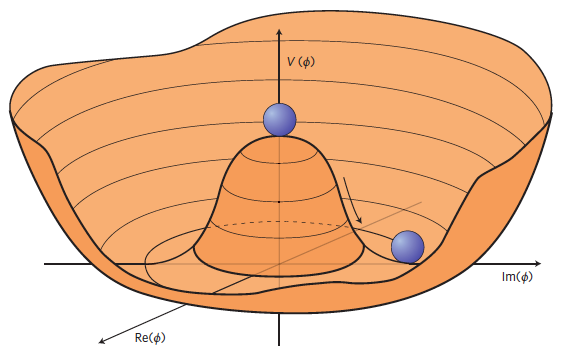
\includegraphics[width=8cm]{figures/ch-1-introduction/higgs-potential.png}
    \caption[An illustration of the Higgs potential.]{An illustration of the Higgs potential \cite{Ellis:2013jnq}. Choosing any of the points at the bottom of the potential breaks spontaneously the rotational $U(1)$ symmetry.}
    \label{fig:higgs-potential}
\end{figure}

The excitations of the Higgs field with respect to the minimum $\Phi_{\text{min}}$ are parameterized by 
\begin{equation}
    \Phi(x) = \exp(i \boldsymbol{\xi}(x) \cdot \boldsymbol{\tau}) \frac{1}{\sqrt{2}} \begin{pmatrix} 0 \\ v + H(x) \end{pmatrix}
\end{equation}
Three degrees of freedom are coupled directly to the electroweak gauge bosons; this is often referred to as the gauge bosons ``eating'' the Goldstone bosons to form the longitudinal polarizations of the massive spin-1 boson states. The $H(x)$ excitation is in the radial direction and corresponds to the free particle state of the Higgs boson. 

\section{Two-Higgs Doublet Models}
\label{section:theory-2HDM}

One of the simplest possible extensions to the Standard Model is adding a doublet to the minimal Higgs sector of the Standard Model, which is a $SU(2)_L$ doublet $H$ with hypercharge $Y = +\frac{1}{2}$, denoted here as $H \sim 2_{+1/2}$. These extensions are found in several theories such as supersymmetry. A general 2HDM can be extended with a light scalar (2HDM+S) to obtain a rich set of exotic Higgs decays \cite{2HDM-PhysRevD.90.075004}. 

The charges of the Higgs fields are chosen to be $H_1 \sim 2_{-1/2}$ and $H_2 \sim 2_{+1/2}$, which acquire vacuum expectation values $v_{1,2}$ which are assumed to be real and aligned \cite{2HDM-PhysRevD.90.075004}. Expanding about the minima yields two complex and four real degrees of freedom:
\begin{align}
    H_1 &= \frac{1}{\sqrt{2}} \begin{pmatrix} v_1 + H^{0}_{1, R} + iH^0_{1, I} \\  
                                              H^-_{1,R} + i H^-_{1, I}   \end{pmatrix} \\
    H_2 &= \frac{1}{\sqrt{2}} \begin{pmatrix} H^+_{2, R} + iH^+_{2, I} \\  
                                              v_2 + H^0_{2,R} + i H^0_{2, I}   \end{pmatrix} 
\end{align}

The charged scalar and pseudoscalar mass matrices are diagonalized by a rotation angle $\beta$, defined as $\tan\beta = v_2/v_1$. One charged (complex) field and one neutral pseudoscalar combination of $H^0_{1, 2, I}$ are eaten by the SM gauge bosons after electroweak symmetry breaking \cite{2HDM-PhysRevD.90.075004}. The other complex field yields two charged mass eigenstates $H^\pm$, which are assumed to be heavy. The remaining three degrees of freedom yield one neutral pseudoscalar mass eigenstate 
\begin{equation}
    A = H^0_{1, I}\sin\beta - H^0_{2, I} \cos\beta
\end{equation}
and two neutral scalar mass eigenstates (where $-\pi/2 \leq \alpha \leq pi/2$)
\begin{equation}
    \begin{pmatrix} h \\ H^0 \end{pmatrix} = \begin{pmatrix} -\sin\alpha & \cos\alpha \\
                                                              \cos\alpha & \sin\alpha \end{pmatrix}
                                             \begin{pmatrix} H^0_{1, R} \\ H^0_{2, R}  \end{pmatrix}
\end{equation}
We assume that the 2HDM is near or in the decoupling limit: $\alpha \rightarrow \pi/2 - \beta$, where the lightest state in the 2HDM is $h$, which we identify as the 125 GeV Higgs particle \cite{2HDM-PhysRevD.90.075004}. In this limit, the fermion couplings of $h$ become identical to the Standard Model Higgs, while the gauge boson couplings are very close to Standard Model-like for $\tan\beta \gtrsim 5$. All of the properties of $h$ are determined by just two parameters: $\tan\beta$ and $\alpha$, and the fermion couplings to the two Higgs doublets. 

2HDM can be extended by a scalar singlet (2HDM+S) \cite{2HDM-PhysRevD.90.075004}:
\begin{equation}
    S = \frac{1}{\sqrt{2}} (S_R + iS_I)
\end{equation}
If this singlet only couples to the Higgs doublets $H_{1,2}$ and has no direct Yukawa couplings, all of its couplings to SM fermions result from mixing with $H_{1,2}$. Under these simple assumptions, exotic Higgs decays $h\rightarrow ss \rightarrow X\bar{X}Y\bar{Y}$ or $h\rightarrow aa \rightarrow X\bar{X}Y\bar{Y}$, and $h \rightarrow aZ \rightarrow X\bar{X}Y\bar{Y}$ are permitted, where $s(a)$ is a (pseudo)scalar mass eigenstate mostly composed of $S_R (S_I)$, and $X, Y$ are Standard Model fermions or gauge bosons. There are two pseudoscalars in the 2HDM+S, and the mostly singlet-like pseudoscalar can be chosen to be the one lighter than the SM-like Higgs. For $m_a < m_h - m_Z \sim 35$ GeV, the exotic Higgs decay $h \rightarrow Za$ is possible, and for $m_a < m_h/2 \approx 63$ GeV, the exotic Higgs decay $h \rightarrow aa$ is possible. 

\begin{figure}[ht]
    \centering
    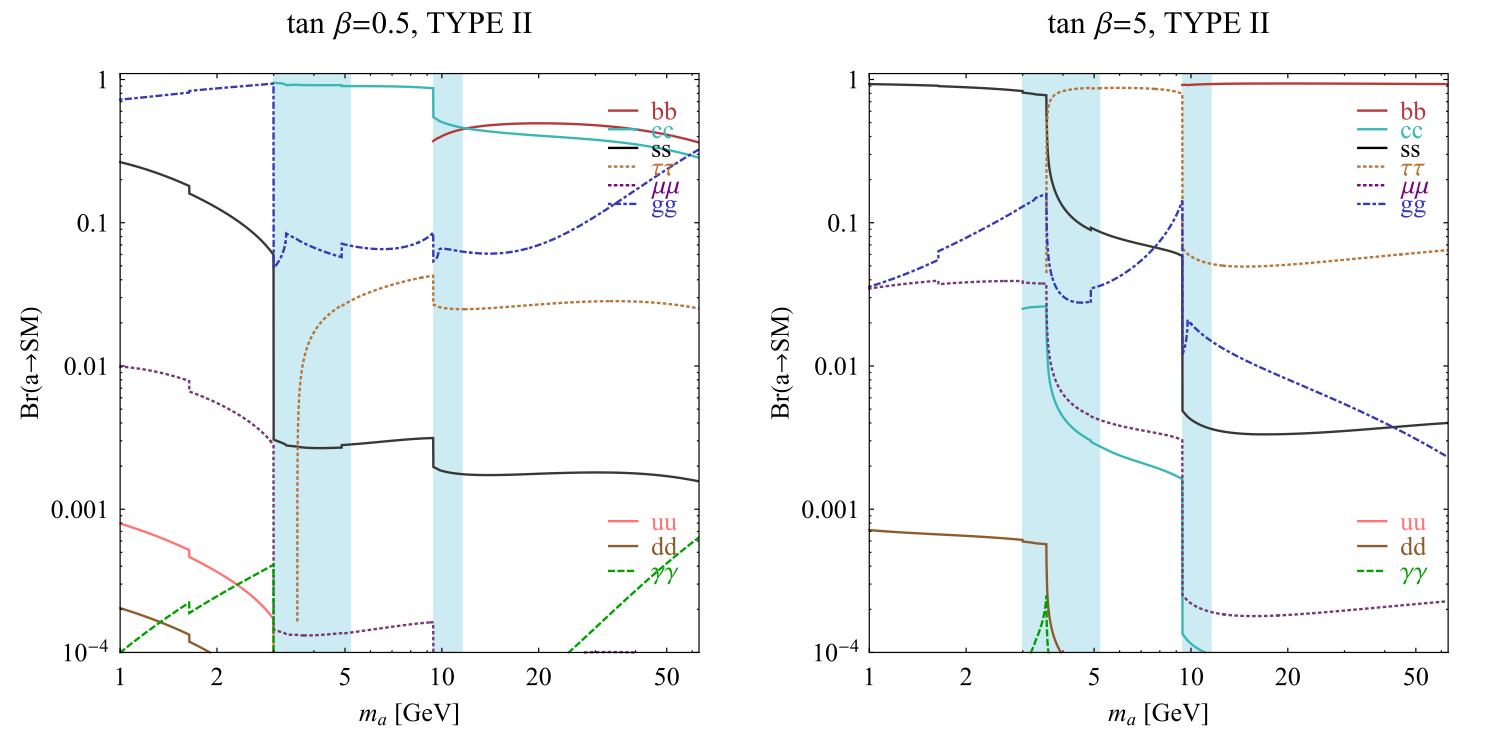
\includegraphics[width=15cm]{figures/ch-1-introduction/curtin-2014-figure-7-BRs-of-singlelike-pseudoscalar-type-II.png}
    \caption[Branching ratios of a singlet-like pseudoscalar in Type II 2HDM+S for $\tan\beta = 0.5$ (left) and $\tan\beta = 5$ (right).]{Branching ratios of a singlet-like pseudoscalar in Type II 2HDM+S for $tan\beta = 0.5$ (\textit{left}) and $\tan\beta = 5$ (\textit{right}) from \cite{2HDM-PhysRevD.90.075004}, showing the dependence of the branching ratios on $\tan\beta$, as well as the prominence of the branching ratios to $bb$ and $\tau\tau$, the channels searched for in the analysis presented here.}
    \label{fig:curtin-2014-fig-4-typeI-BRs}
\end{figure}


In 2HDM, and by extension 2HDM+S, there are four types of fermion couplings commonly discussed in the literature that forbid flavor-changing neutral currents at tree level \cite{2HDM-PhysRevD.90.075004}. These are referred to as Type I (all fermions couple to $H_2$), Type II (MSSM-like, $d_R$ and $e_R$ couple to $H_1$, $u_R$ to $H_2$), Type III (lepton-specific, leptons and quarks couple to $H_1$ and $H_2$ respectively) and Type IV (flipped, with $u_R$, $e_R$ coupling to $H_2$ and $d_R$ to $H_1$). The exact branching ratios of the pseudoscalars to Standard Model particles vary depending on the 2HDM+S model and the value of $\tan\beta$ (e.g. Fig. \ref{fig:curtin-2014-fig-4-typeI-BRs}).

\section{Two Real Singlet Model}
\label{section:theory-TRSM}
The two real singlet model (TRSM) adds two real singlet degrees of freedom to the Standard Model. These are written as two real singlet fields $S$ and $X$. Depending on the vacuum expectation values acquired by the scalars, different phases of the model can be realized \cite{Robens:2019kga}. To reduce the number of free parameters, two discrete $\mathbb{Z}_2$ symmetries are introduced. The fields are decomposed as

\begin{equation}
    \Phi = \begin{pmatrix} 0 \\ \frac{\phi_h + v}{\sqrt{2}} \end{pmatrix}, 
    \,
    S = \frac{\phi_S + v_S}{\sqrt{2}} ,
    \,
    X = \frac{\phi_X + v_X}{\sqrt{2}}
\end{equation}
To achieve electroweak-breaking symmetry, $v  = v_{SM} \sim 246$ 246 GeV is necessary. If the vacuum expectation values $v_S, v_X \neq 0$ the $\mathbb{Z}_2$ are spontaneously broken, and the fields $\phi_{h,S,X}$ mix into three physical scalar states. This is called the broken phase and leads to the most interesting collider phenomenology.

The mass eigenstates $h_{1,2,3}$ are related to the fields $\phi_{h,S,X}$ through a $3\times 3$ orthogonal mixing matrix denoted $R$. The mass eigenstates are assumed to be ordered $M_1 \leq M_2 \leq M_3$. $R$ is parameterized by the three mixing angles $\theta_{hS}$, $\theta_{hX}$, $\theta_{SX}$. The nine parameters of the scalar potential can be expressed in terms of the three physical Higgs masses, the three mixing angles, and the three vacuum expectation values. 

After fixing one of the Higgs masses to the mass of the observed Higgs boson, and fixing the Higgs doublet vacuum expectation value to its Standard Model value, there are seven remaining free parameters of the TRSM \cite{Robens:2019kga}.

In one benchmark scenario of TRSM \cite{Robens:2019kga}, the heaviest scalar state $h_3$ is identified with the 125 GeV Higgs, $h_{125}$, and it can decay asymmetrically $h_{125} \rightarrow h_1 h_2$, which we also denote $h \rightarrow a_1 a_2$ to highlight the similarity with the symmetric decay $h \rightarrow aa$ typically interpreted in 2HDM+S as discussed. The parameter values in TRSM are chosen such that the coupling of $h_3$ to Standard Model particles are nearly identical to the Standard Model predictions. 

\begin{figure}[ht]
    \centering
    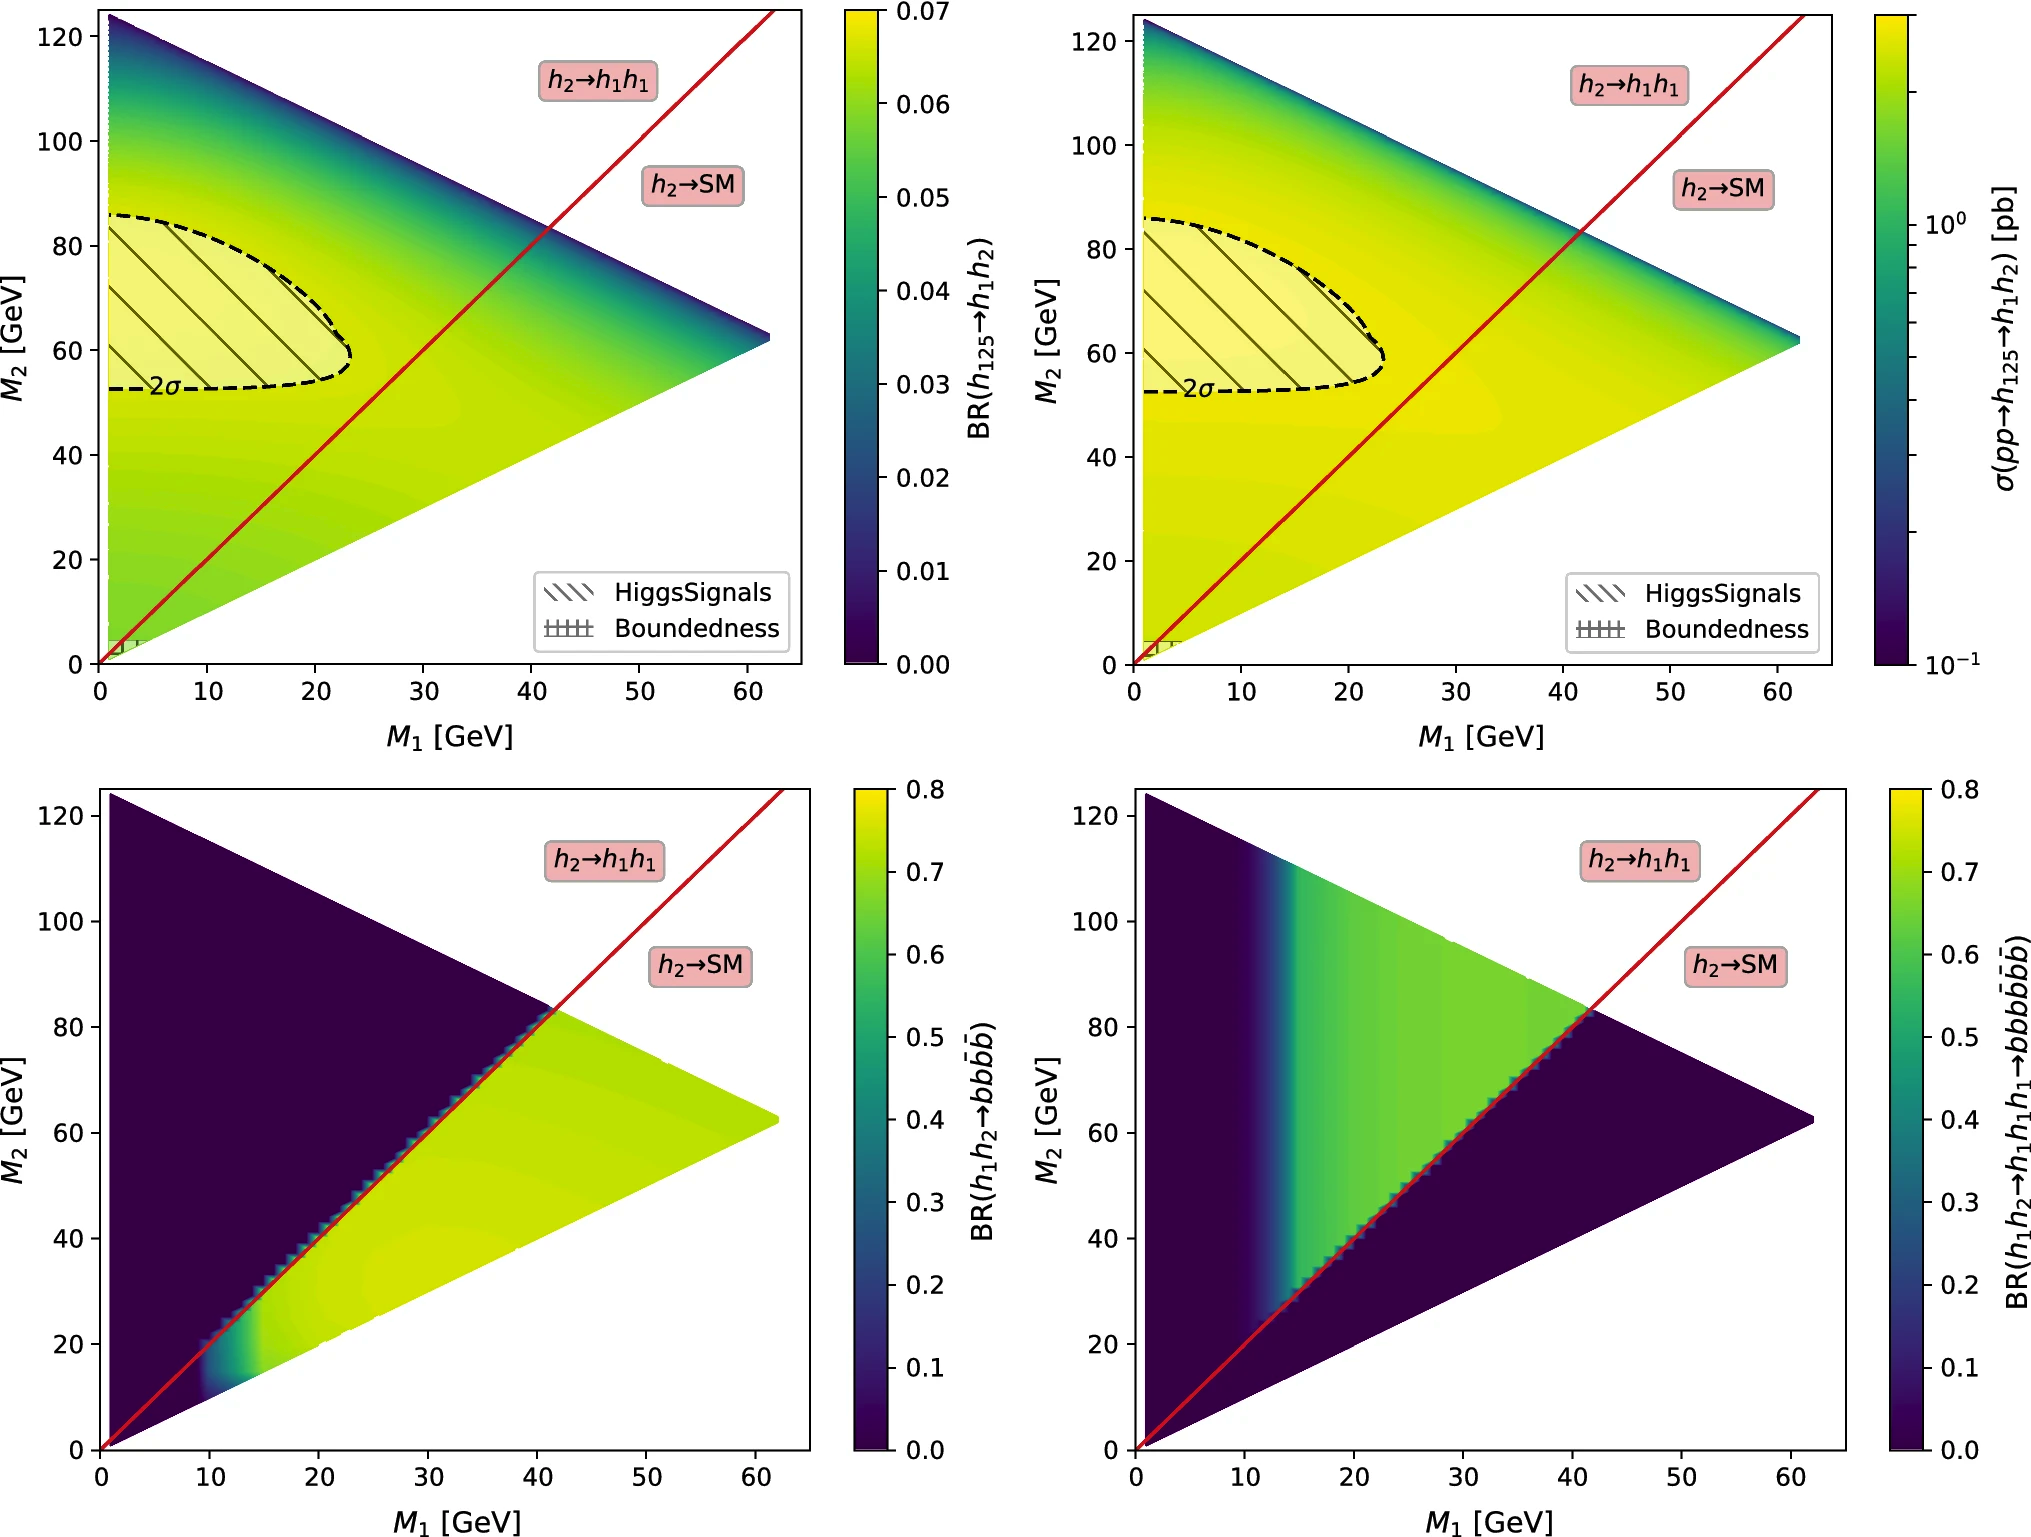
\includegraphics[width=15cm]{figures/ch-1-introduction/Robens-TRSM-Figure-6-BP-1.png}
    \caption[Benchmark plane BP1 for benchmark scenario 1, for the decay signature $h_{125} \rightarrow h_1 h_2$ with $h_{125} \equiv h_3$, defined in the $(M_1, M_2)$ plane.]{Benchmark plane BP1 for benchmark scenario 1 from \cite{Robens:2019kga}, for the decay signature $h_{125} \rightarrow h_1 h_2$ with $h_{125} \equiv h_3$, defined in the $(M_1, M_2)$ plane. The color code shows BR$(h_3 \rightarrow h_1 h_2)$ (\textit{top left}) and the 13 TeV LHC signal rate for $pp \rightarrow h_3 \rightarrow h_1 h_2$ (\textit{top right}). The red line separates the region $M_2 > 2 M_1$, where BR($h_2 \rightarrow h_1 h_1$) $\sim 100\%$, from the region $M_2 < 2 M_1$, where BR($h_2 \rightarrow F_{SM}$) $\sim 100\%$. The \textit{bottom left} and \textit{right} show the branching ratio of the $h_1 h_2$ into (respectively) $b\bar{b}b\bar{b}$, and through a $h_2 \rightarrow h_1 h_1$ cascade to $b\bar{b}b\bar{b}b\bar{b}$. The hatched region indicates where the decay rate slightly exceeds the $2\sigma$ upper limit inferred from the LHC Higgs rate measurements, though the region depends on the parameter choices and experimental searches should cover the whole mass range.}
    \label{fig:trsm_bp1}
\end{figure}

In benchmark scenario 1 (benchmark plane 1, or BP1) (Fig. \ref{fig:trsm_bp1}) \cite{Robens:2019kga}, the maximal branching ratios for $h_3 \rightarrow h_1 h_2$ reach up to $7-8\%$ which translates into a signal rate of around 3 pb. These maximal branching ratios are reached in the intermediate mass state for $h_2$, $M_2 \sim 60 - 80$ GeV. For $M_2 < 40$ GeV, although phase space opens up significantly for light decay products, the branching ratio becomes smaller. 

If the decay channel $h_2 \rightarrow h_1 h_1$ is kinematically open (i.e. $M_2 > 2M_1$), it is the dominant decay mode leading to a significant rate for the $h_1 h_1 h_1$ final state, in a ``cascade" decay. In BP1, $BR(h_2 \rightarrow h_1h_1$) $\simeq 100\%$ above the red line in Fig. \ref{fig:trsm_bp1}. If, in addition, $M_1 \gtrsim 10$ GeV, the $h_1$ decays dominantly to $b\bar{b}$ leading to a sizable rate for the $b\bar{b}b\bar{b}b\bar{b}$ final state as shown in Fig. \ref{fig:trsm_bp1} (\textit{bottom right}).

If the $h_2 \rightarrow h_1 h_1$ decay is kinematically closed (i.e. $M_2 < 2M_1$), both scalars decay directly to Standard Model particles, with branching ratios identical to a Standard Model-like Higgs boson, i.e. with the $b\bar{b}b\bar{b}$ final state dominating, as shown in Fig. \ref{fig:trsm_bp1} (\textit{bottom left}), while at smaller masses, combinations with $\tau$ leptons and eventually final states with charm quarks and muons become relevant \cite{Robens:2019kga}.


\chapter{The Large Hadron Collider and the CMS Experiment}
This chapter introduces the key aspects of the CERN Large Hadron Collider (LHC) and the Compact Muon Solenoid (CMS) experiment where the work for this thesis was conducted. Section \ref{section:LHC} describes the history of accelerator developments at CERN that led to the construction of the LHC, the current LHC configuration, and the largest experiments located at the LHC. The concepts of beam luminosity and pileup, which are critical for understanding and measuring high-energy particle collisions, are described in Section \ref{section:luminosity_and_pileup} and discussed in the context of the High-Luminosity LHC (HL-LHC) upgrade in Section \ref{section:HL-LHC}. Lastly, Section \ref{section:cms-detector} describes the design and function of CMS and its subdetectors, and terminates in a description of data processing at CMS, beginning from online event filtering in the Level-1 Trigger, to processing in the High-Level Trigger, to offline particle reconstruction, and finally long-term storage and processing of measured events.

\section{The Large Hadron Collider}
\label{section:LHC}
CERN, the European Organization for Nuclear Research, is an international organization based in Meyrin, Switzerland which operates the world's largest particle physics laboratory, and is the site of the Large Hadron Collider (LHC) \cite{history_of_CERN}. The very first accelerator built at CERN was the 600 MeV Synchrocyclotron (SC), which initially provided beams for CERN's first experiments. The newer and more powerful Proton Synchrotron (PS), which could accelerate particles to an energy of 28\GeV, began operations in 1959 and is still in use today. The first hadron collider at CERN was the Intersecting Storage Rings (ISR), which consisted of two interlaced rings each with a diameter of 200. The ISR collided protons at a center-of-mass energy of 62\GeV and began measuring collisions in 1971. In 1968 CERN began to accelerate heavy ions in the Super Proton Synchrotron (SPS), which is 7 kilometers in circumference and was the first of CERN's giant underground rings to be built. The SPS became the forefront of CERN's particle physics program in 1976, and in 1981 was converted into a proton-antiproton collider. The final and largest underground ring constructed at CERN was the Large Electron-Positron (LEP) collider, which was commissioned in July 1989 and hosted 5176 magnets and 128 accelerating cavities located around a 27-kilometer circumference. Over 11 years of research, four detectors, ALEPH, DELPHI, L3, and OPAL measured the collisions, with collision energies reaching up to 209\GeV in the year 2000. In November 2000, LEP was closed down to make way for the construction of the LHC in the same tunnel.

In its current configuration, the LHC accelerator complex at CERN is a succession of machines that accelerate particles in stages until they reach their final energy of 6.5 TeV per beam \cite{CERN-OPEN-2000-148} \cite{Linac4-design-report-2020}. In Linear accelerator 4 (Linac4), negative hydrogen ions (hydrogen atoms with an additional electron) are accelerated to 160 MeV, and stripped of their two electrons, leaving only protons, before entering the Proton Synchrotron Booster (PSB). These protons are accelerated to 2\GeV, then to 26\GeV in the Proton Synchrotron (PS), and 450\GeV in the Super Proton Synchrotron (SPS). The protons are transferred to the two beam pipes of the Large Hadron Collider (LHC). The LHC is a 27-kilometer ring of superconducting magnets, inside which one beam circulates clockwise and the other counterclockwise. Each LHC ring takes 4 minutes and 20 seconds to fill, and it takes about 20 minutes for the protons to reach their maximum energy. During normal operating conditions, beams circulate for many hours inside the LHC ring. 

The beams of particles in the LHC are made to collide at a center-of-mass energy of up to 14 TeV, at four positions at particle detector experiments located around the ring: ATLAS, CMS, ALICE, and LHCb. An aerial view of the four major experiments' locations is shown in Fig. \ref{fig:aerial-view-LHC-ring} \cite{OPEN-PHO-ACCEL-2017-005}. ATLAS and CMS are the two general-purpose detectors with broad physics programmes spanning Standard Model measurements and searches for signatures of new physics \cite{ATLAS-TDR-14} \cite{CERN-LHCC-2006-001}. The two experiments use different technical solutions and different magnet system designs. ALICE is a general-purpose detector dedicated to measuring LHC heavy-ion collisions, and is designed to address the physics of strongly interacting matter, and the properties of quark-gluon plasma \cite{ALICE-original-TDR}. The LHCb experiment specializes in investigating CP violation through measuring the differences in matter and antimatter, by using a series of subdetectors to detect mainly forward particles close to the beam direction \cite{LHCb-1998}. 

\begin{figure}[ht]
    \centering
    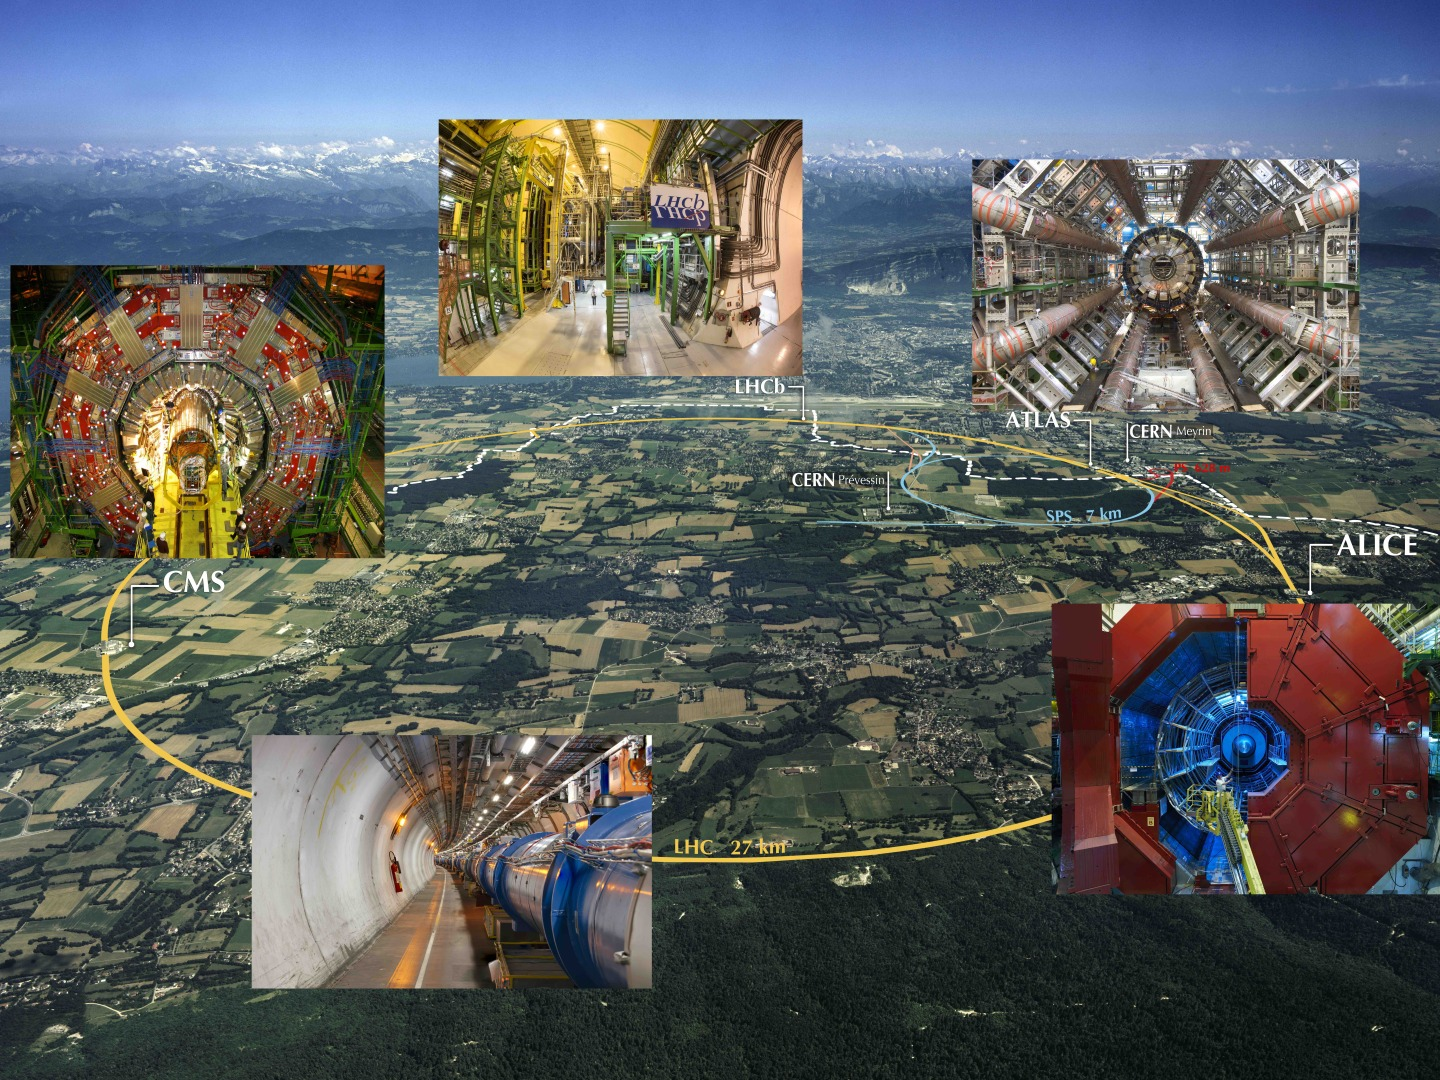
\includegraphics[width=11cm]{figures/ch-2-cern-cms/aerial-view-LHC-ring.jpeg}
    \caption[Aerial view of the Large Hadron Collider (LHC).]{Aerial view of the Large Hadron Collider (LHC) spanning the border of France and Switzerland, and the four major experiments located around the ring: CMS (Compact Muon Solenoid), LHCb (LHC beauty), ATLAS (A Toroidal LHC Apparatus), and ALICE (A Large Ion Collider Experiment) \cite{OPEN-PHO-ACCEL-2017-005}.}
    \label{fig:aerial-view-LHC-ring}
\end{figure}



\section{Luminosity and pileup}
\label{section:luminosity_and_pileup}
In order to search for rare decays, such as those that result from the creation and decay of a Higgs, W, or Z boson, a large number of parton interactions per second are required at the LHC. The number of events generated per second by the LHC collisions is given by
\begin{equation}
     N_{event} = \mathcal{L} \cdot \sigma_{event}
    \label{eqn:nEvents}
\end{equation} 
where $\sigma_{event}$ is the cross-section for the event under study, and $\mathcal{L}$ the instantaneous luminosity. The instantaneous luminosity is measured in units of cm$^{-2}$ s$^{-1}$, and depends only on the beam parameters, and can be written for a Gaussian beam distribution as:
\begin{equation}
    \mathcal{L} = \frac{N_b^2 n_b f_{rev} \gamma_r}{4\pi \epsilon_n \beta^*} F
\end{equation}
where the parameters are as defined, along with some example typical nominal values in Phase-1 of the LHC \cite{CERN-luminosity-accelerator-school-article} \cite{ipac2012-proceedings}:
% reference: material included in introduction to accelerator physics 2021 https://indico.cern.ch/event/1001431/contributions/

\begin{itemize}
    \item $N_b$ is the number of particles per bunch ($N_b \approx 1.15 \times 10^{11}$ protons per bunch)
    \item $n_b$ is the number of bunches per beam (maximum 2808),
    \item $f_{rev}$ is the revolution frequency ($\approx 11$ kHz),
    \item $\gamma_r$ is the relativistic gamma factor,
    \item $\epsilon_n$ is the normalized transverse beam emittance (area in a transverse plane occupied by the beam particles),
    \item $\beta^*$ is the beta function at the collision point ($\beta^* = 0.55$ m),
    \item and $F$ is the geometric luminosity reduction factor due to the crossing angle at the interaction points ($F \approx 0.84$ for Phase-1. Note that complete overlap would give $F = 1$).
\end{itemize}
Peak luminosity at interaction points 1 and 5 reach values of $\sim 1.0 \times 10^{34}$ cm$^{-2}$ s$^{-1}$, with peak luminosity per bunch crossing reaching $\sim 3.56 \times 10^{34}$ cm$^{-2}$ s$^{-1}$.

Per Eqn. \ref{eqn:nEvents}, the integrated luminosity over time is proportional to the number of events produced, and the size of LHC datasets is commonly presented in terms of integrated luminosity. Collider operation aims to optimize the integrated luminosity. Thus the exploration of rare events in the LHC collisions requires both high beam energies and high beam intensities.

The LHC's nominal beam luminosities are sufficiently large for multiple proton-proton collisions to occur in the same time window of 25 nanoseconds in which proton bunches collide \cite{CMS-JME-18-001}. These multiple collisions will lead to particle interactions overlapping in the detector. To measure a proton-proton collision, the single collision must be separated from overlapping collisions, which are called ``pileup'' collisions. A distribution of pileup in the data-taking years 2016-2018 is shown in Fig. \ref{fig:pileup-run-2}. The pileup is defined as the average number of $pp$ collisions per bunch crossing.

CMS reports an inelastic $pp$ cross section of $\sigma_{\text{inel}} = 68.6$ millibarns at a center-of-mass energy of $\sqrt{s} = 13$ TeV \cite{CERN-EP-2018-004-pileup}, which can be used to estimate pileup as follows:
\begin{equation}
    \text{Pileup} = \frac{\mathcal{L} \times \sigma_{\text{inel}}}{ n_b \cdot f}
\end{equation}
With the example values above, pileup can be estimated to be $\sim 22$.

Thus, higher luminosities create more intense pileup conditions, posing a greater challenge to detector performance and particle reconstruction and identification.

\begin{figure}[ht]
    \centering
    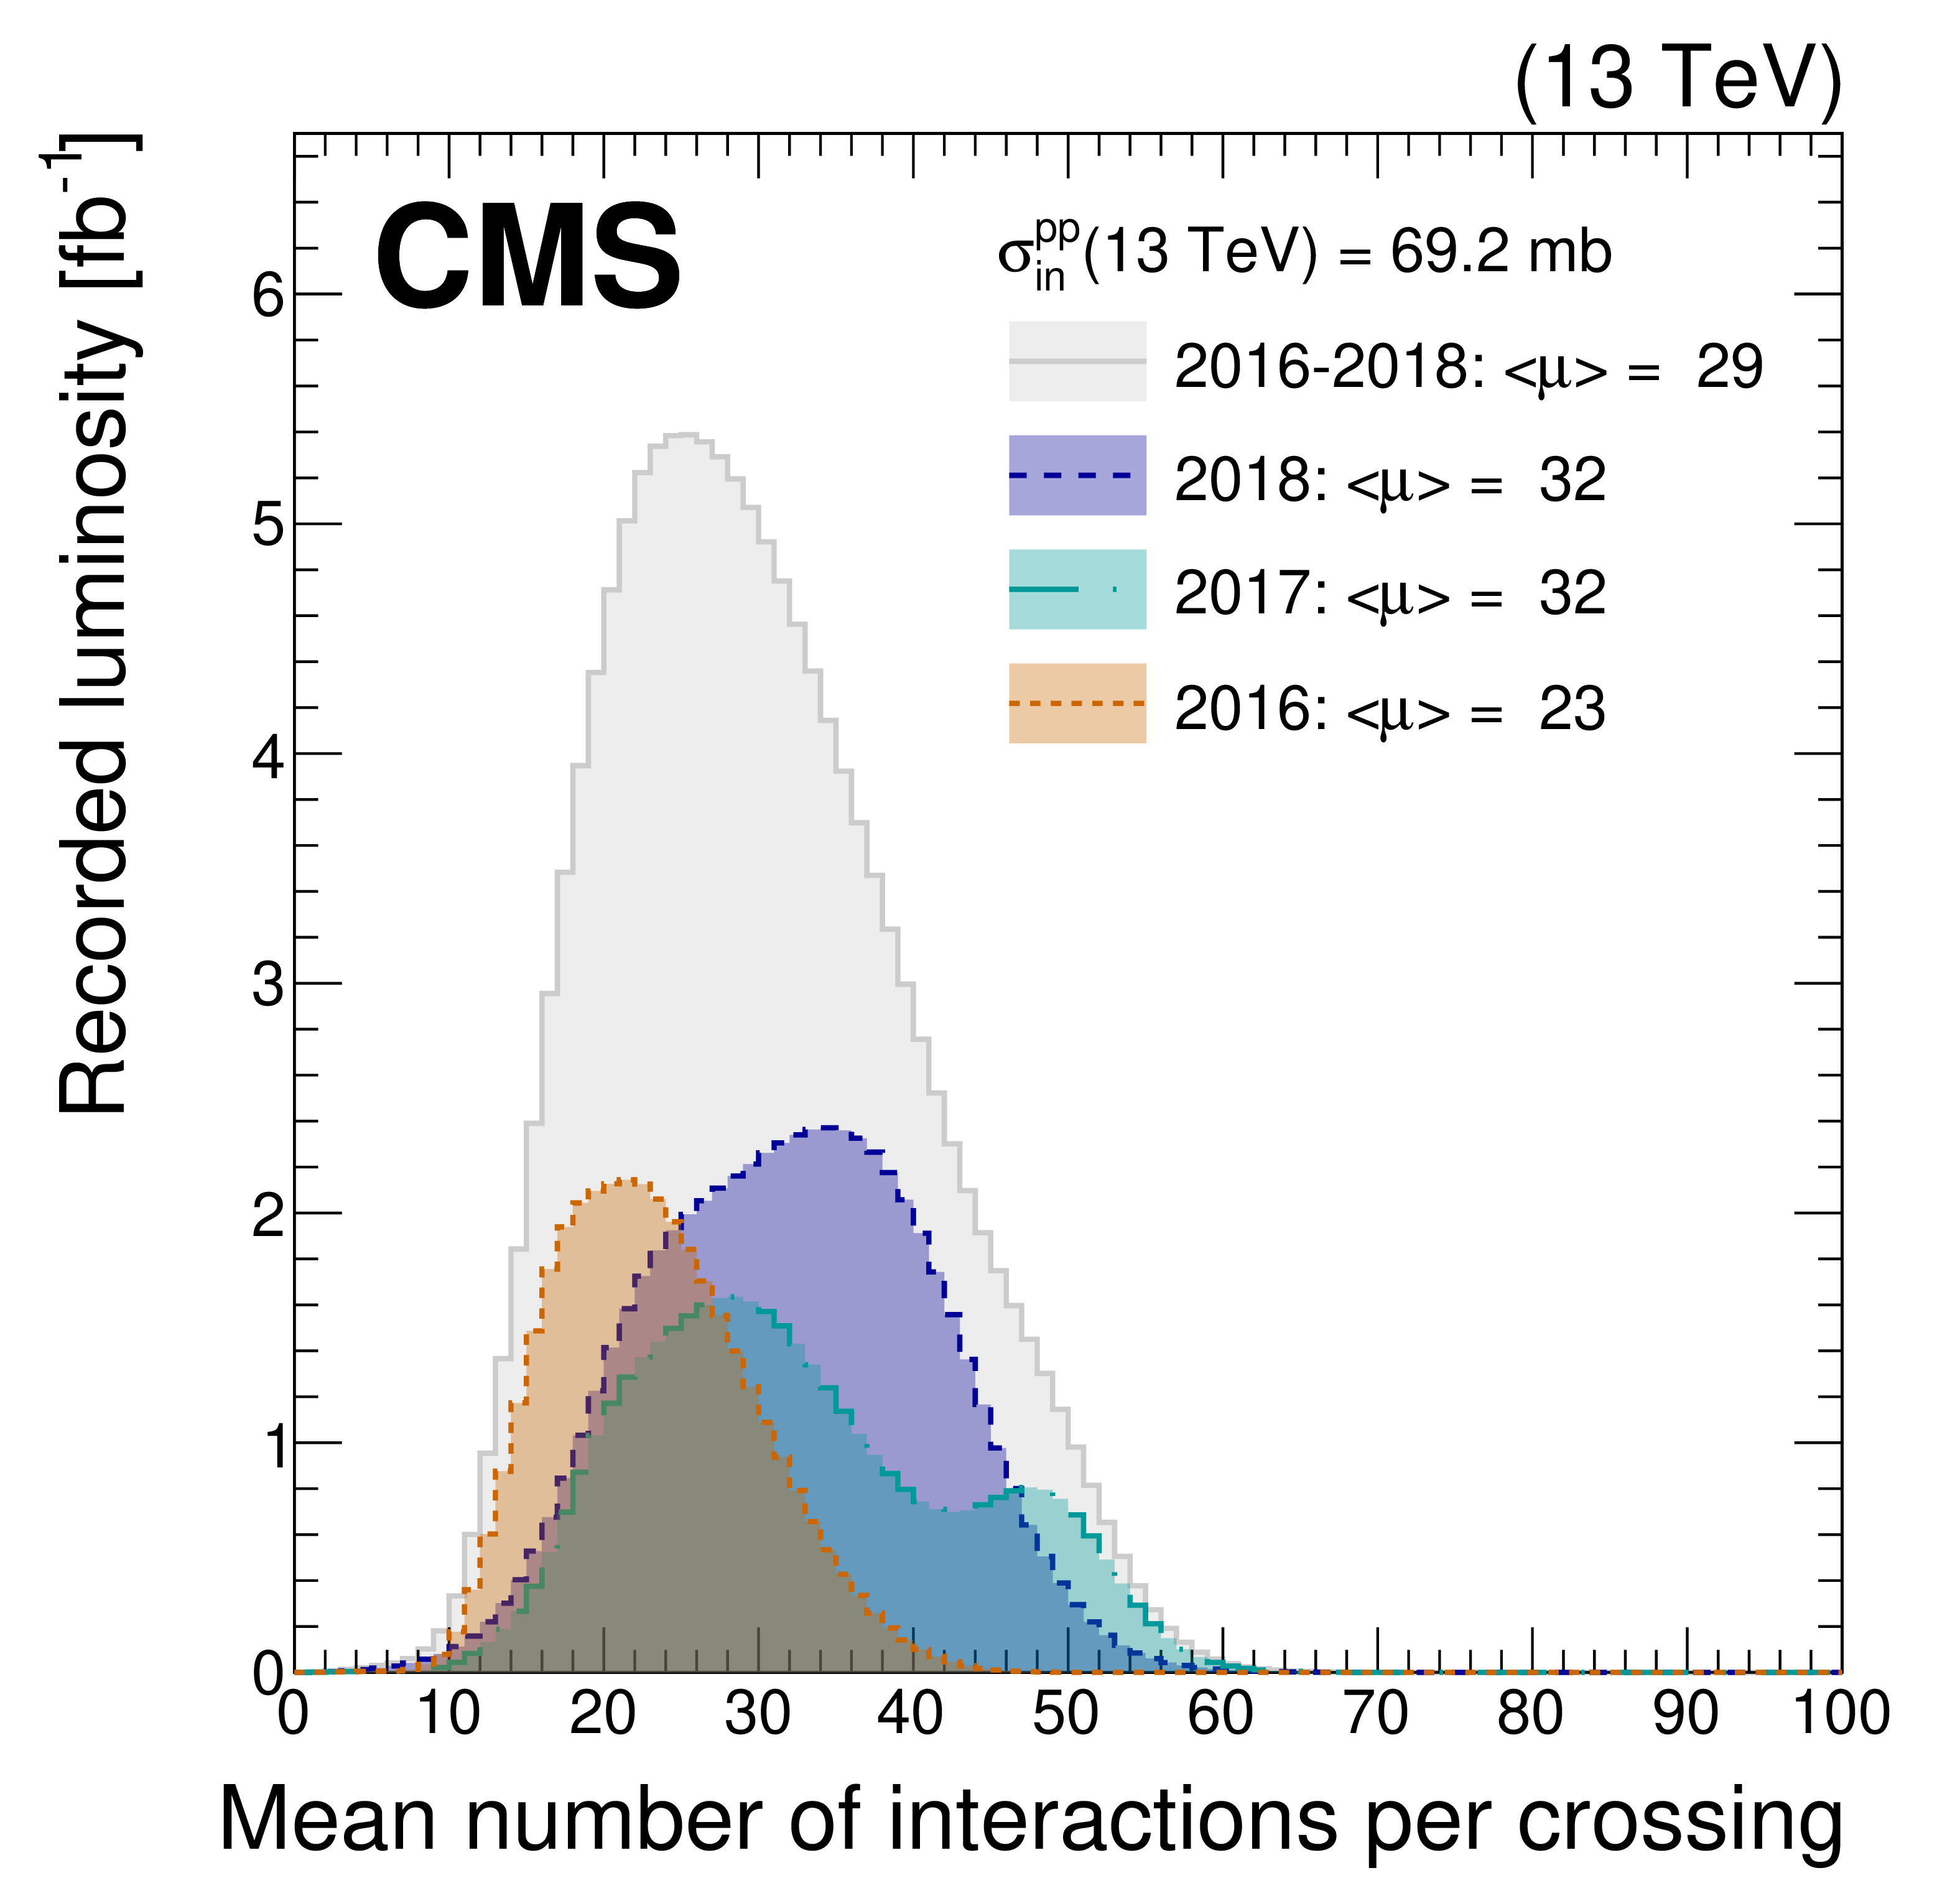
\includegraphics[width=8cm]{figures/ch-2-cern-cms/pileup-run-2-CMS-JME-18-001_Figure_001.png}
    \caption[Distribution of the mean number of inelastic collisions per bunch crossing (pileup) in data, for proton-proton collisions in 2016-2018]{Distribution of the mean number of inelastic collisions per bunch crossing (pileup) in data \cite{CMS-JME-18-001}, for proton-proton collisions in 2016 (\textit{dotted orange}), 2017 (\textit{dotted light blue}), 2018 (\textit{dotted dark blue}), and integrated over 2016-2018 (\textit{solid grey}). A cross-section of inelastic proton-proton collisions of 69.2 mbarns is assumed. In the running conditions of the High-Luminosity LHC, pileup will reach unprecedented levels of up to 200 per bunch crossing \cite{CERN-2020-010-HL-LHC-TDR}.}
    \label{fig:pileup-run-2}
\end{figure}

\section{The High-Luminosity LHC}
\label{section:HL-LHC}
The High-Luminosity LHC (HL-LHC) is a major upgrade of the LHC scheduled to take place in the late 2020s, that will increase the instantaneous luminosity by a factor of of five beyond the original design value, and the integrated luminosity by a factor of ten \cite{CERN-2020-010-HL-LHC-TDR}. This will be accomplished through accelerator technological advances: for instance, reduction of the interaction point $\beta^*$ from 0.55 m down to 0.15 m by installation of new final-focusing magnets, and improvements in the geometric luminosity loss factor $F \approx 1$ through the installation of crab cavities that optimize the orientation of colliding bunches. A further discussion of the HL-LHC upgrades for the CMS detector follows in Chapter \ref{chapter:ch-3:phase-2-upgrade-cms}.

\section{The CMS Detector}
\label{section:cms-detector}

The Compact Muon Solenoid (CMS) experiment was conceived to study proton-proton and lead-lead collisions at a center-of-mass energy of 14 TeV (5.5 TeV nucleon-nucleon) and at luminosities up to $10^{34}$ cm$^{-2}$ s$^{-1}$ ($10^{27}$ cm$^{-2}$ s$^{-1}$) \cite{CMS-2008-JINST-3-S08004} \cite{CERN-EP-2017-110}. Starting from the beam interaction region at the center of the CMS detector, particles first pass through a silicon pixel and strip tracker, in which charged-particle trajectories (tracks) and origins (vertices) are reconstructed from signals (hits) in the sensitive layers. The tracker is immersed in a high-magnetic-field superconducting solenoid that bends the trajectories of charged particles, allowing the measurement of their electric charge and momenta. Electrons and photons are then absorbed in an electromagnetic calorimeter (ECAL) comprised of lead-tungstate scintillating-crystals. The corresponding electromagnetic showers are detected as clusters of energy recording in neighboring cells, from which the direction and energy of the particles can be determined. Charged and neutral hadrons may initiate a hadronic shower in the ECAL as well, which is then fully absorbed in the hadron calorimeter (HCAL). The resulting clusters are used to estimate their direction and energies. Muons and neutrinos pass through the calorimeters with little to no interactions. Neutrinos escaped undetected; muons produce hits in additional gas-ionization chamber muon detectors housed in the iron yoke of the flux-return. A sketch of example particle interactions in a transverse slice of the CMS detector is shown in Fig. \ref{fig:sketch-cms-particle-interactions}. The collision data is recorded with the use of the Level-1 (L1) trigger (discussed in greater detail in \ref{section:phase-1-l1-trigger}), the High-Level Trigger (HLT), and data acquisition systems ensuring high efficiency in selecting physics events of interest. 

\begin{figure}[ht]
    \centering
    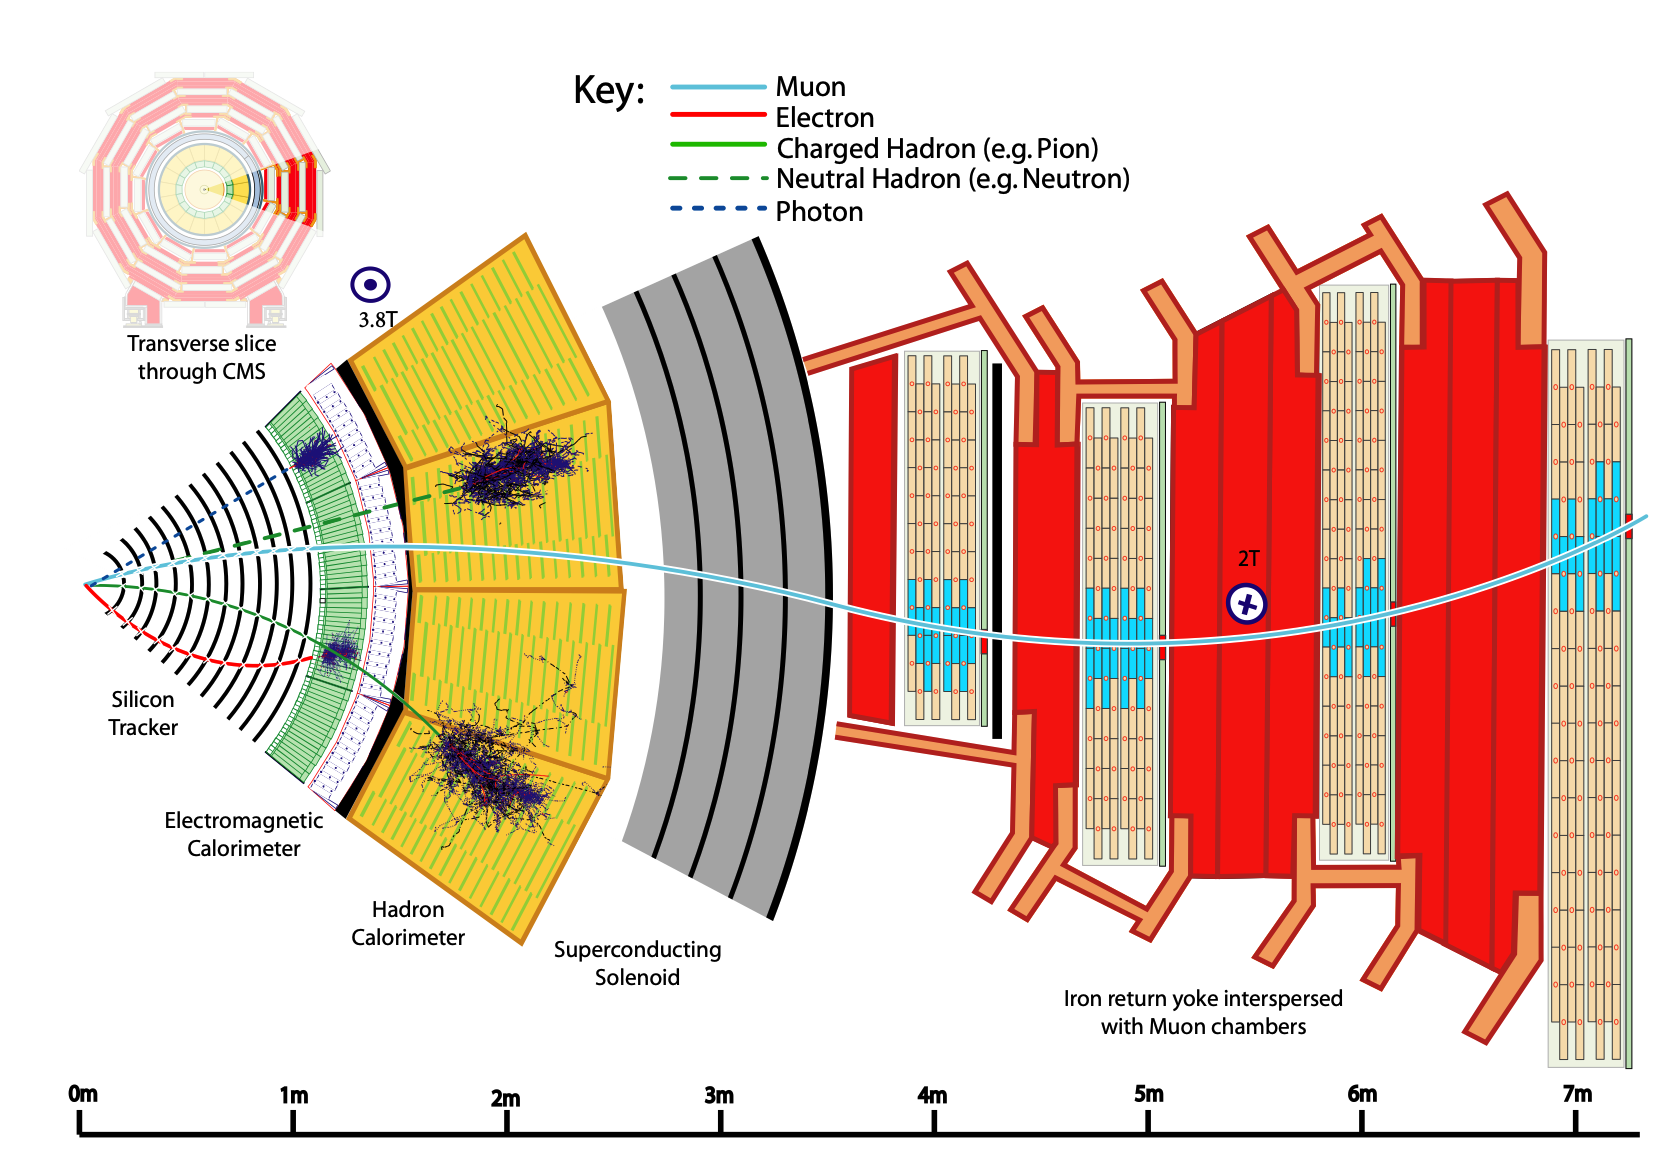
\includegraphics[width=11cm]{figures/ch-2-cern-cms/sketch-cms-particle-interactions.png}
    \caption[Sketch of particle trajectories of muons, electrons, charged and neutral hadrons, and photons in a transverse cross-section of the CMS detector.]{Sketch of particle trajectories of muons, electrons, charged and neutral hadrons, and photons in a transverse cross-section of the CMS detector \cite{CERN-EP-2017-110}.}
    \label{fig:sketch-cms-particle-interactions}
\end{figure}

CMS uses a right-handed coordinate system \cite{CMS-2008-JINST-3-S08004}. The origin is centered at the nominal collision point inside the experiment. The $x$ axis points towards the center of the LHC, and the $y$ axis points vertically upwards. The $z$ axis points along the beam direction. The azimuthal angle, $\phi$, is measured from the $x$ axis in the $x$-$y$ plane, and the radial coordinate in this plane is denoted by $r$. The polar angle, $\theta$, is measured from the $z$ axis. The pseudorapidity, $\eta$, is defined as $\eta = -\ln \tan(\theta/2)$. The momentum and energy transverse to the beam direction, denoted by $p_{T}$ and $E_{T}$ respectively, are computed from the $x$ and $y$ components. The momentum imbalance in the transverse plane is called the missing transverse momentum, and its magnitude is denoted by $E_{T}^{\text{miss}}$.

\section{Sub-detectors of CMS}
This section details the sub-detectors of CMS that operate to identify and precisely measure muons, electrons, photons, and jets over a large energy range. 

\subsection{Inner tracking system}

The CMS Tracker performs robust tracking and detailed vertex reconstruction in the 4 T magnetic field of the superconducting solenoidal magnet. The primary sensors used in the tracker are $p^+$ on $n$-bulk devices, which allow high voltage operation and are radiation-resistant \cite{CERN-LHCC-98-006} \cite{CERN-LHCC-2017-009-tracker-phase2-tdr}. The active envelope of the CMS Tracker extends to a radius of 115 cm, over a length of approximately 270 cm on each side of the interaction point \cite{CERN-LHCC-98-006}.
Charged particles in the region $|\eta| \lesssim 1.6$ benefit from the full momentum measurement precision. In this region, a charged particle with $p_T$ of 1000\GeV has a sagitta of $\sim 195$ $\mu$m. The Tracker acceptance extends further to $|\eta| = 2.5$, with a reduced radius of approximately 50 cm.

The high magnetic field of CMS causes low $p_{T}$ charged particles to travel in helical trajectories with small radii. The majority of events contain particles with a steeply falling $p_{T}$ spectrum, resulting in a track density which rapidly decreases at higher radii. 

A schematic view of the current Phase-1 CMS tracker \cite{CMS-TDR-011-pixel}, including the pixel detector, is shown in Fig. \ref{fig:phase-1-tdr-tracker-schematic}. The Phase-1 pixel detector consists of three barrel layers (BPIX) at radii of 4.4 cm, 7.3 cm, and 10.2 cm, and two forward/backward disks (FPIX) at longitudinal positions of $\pm$ 34.5 cm and $\pm$ 46.5 cm, and extending in radius from about 6 cm to 15 cm. These pixelated detectors produce 3D measurements along the paths of charged particles with single hit resolutions between 10-20 $\mu$m. 


\begin{figure}[ht]
    \centering
    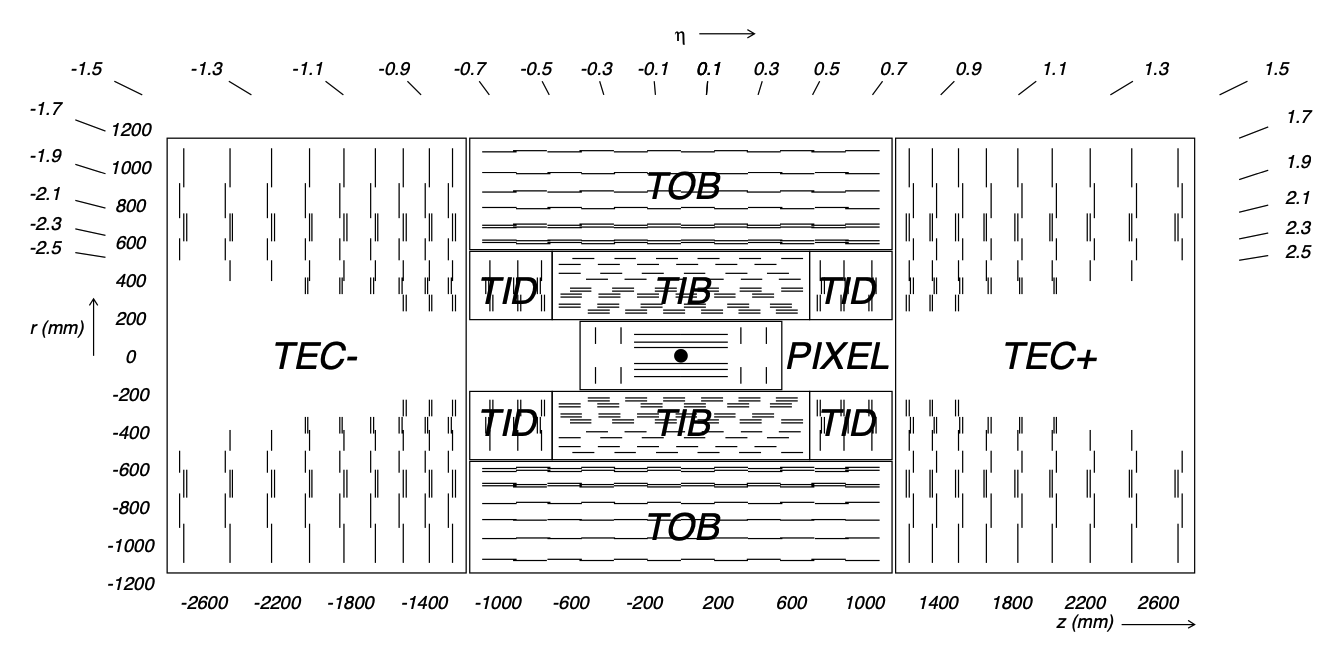
\includegraphics[width=11cm]{figures/ch-2-cern-cms/phase-1-tdr-tracker-schematic.png}
    \caption[Cross section of the current Phase-1 CMS tracker.]{Cross section of the current Phase-1 CMS tracker \cite{CMS-TDR-011-pixel}. Each line represents a detector module. Double lines indicate back-to-back modules which deliver two-dimensional (stereo) hits in the strip tracker.}
    \label{fig:phase-1-tdr-tracker-schematic}
\end{figure}

After the pixel and on their way out of the tracker, particles pass through the silicon strip tracker which reaches out to a radius of 130 cm (Fig. \ref{fig:phase-1-tdr-tracker-schematic}). The sensor elements in the strip tracker are single-sided $p$-on-$n$ type silicon micro-strip sensors \cite{CMS-2008-JINST-3-S08004}. The silicon strip detector consists of four inner barrel (TIB) layers assembled in shells, with two inner endcaps (TID), each composed of three small discs. The outer barrel (TOB) consists of six concentric layers. Two endcaps (TEC) close off the tracker on either end. 


\subsection{ECAL} 
The electromagnetic calorimeter (ECAL) of CMS measures electromagnetic energy deposits with high granularity. One of the driving criteria in the design was the capability of detecting the Standard Model Higgs boson decay to two photons (in fact, the channel in which the 125\GeV Higgs boson was discovered at CMS). 
ECAL is a hermetic homogeneous calorimeter comprised of 61,200 lead tungstate (PbWO$_4$) crystals mounted in the central barrel, with 7,324 crystals in each of the two endcaps \cite{CMS-2008-JINST-3-S08004}. A preshower detector is located in front of the endcap crystals. Avalanche photodiodes (APDs) are used as photodetectors in the barrel and vacuum phototriodes (VPTs) in the endcaps. 

The design of the ECAL is driven by the behaviour of high-energy electrons, which predominantly lose energy in matter via bremsstrahlung, and high-energy photons by $e^+ e^-$ pair production. The characteristic amount of matter traversed for these interactions is the radiation length $X^0$, usually measured in units of g cm$^-2$. The radiation length is also the mean distance over which a high-energy electron loses all but $1/e$ of its energy via bremsstrahlung \cite{workman_review_2022}. Thus high granularity in $\eta$ and $\phi$, and the length of the ECAL crystals, is designed to capture the shower of $e/\gamma$ produced by electrons and photons.

The barrel part of the ECAL (EB) covers the pseudorapidity range $|\eta| < 1.479$ \cite{CMS-2008-JINST-3-S08004}. The barrel granularity is 360-fold in $\phi$ and ($2 \times 85$)-fold in $\eta$. The crystal cross-section corresponds to approximately $0.0174 \times 0.0174$ in $\eta-\phi$ or $22 \times 22$ mm$^2$ at the front face of the crystal, and $26 \times 26$ mm$^2$ at the rear face. The crystal length is 230 mm, corresponding to 25.8 $X_0$.

The ECAL read-out acquires the signals of the photodetectors  \cite{CMS-2008-JINST-3-S08004}. At each bunch crossing, digital sums representing the energy deposit in a trigger tower, comprising $5 \times 5$ crystals in $\eta \times \phi$, are generated and sent to the Level-1 trigger system (detailed in Section \ref{section:phase-1-l1-trigger}).

\subsection{HCAL}
The hadronic calorimeter (HCAL) of CMS measures hadronic energy, which is key to characterizing the presence of apparent missing transverse energy which could arise from hadron jets and neutrinos or exotic particles \cite{CMS-2008-JINST-3-S08004}. A schematic of the components of HCAL are shown in Fig. \ref{fig:phase-1-HCAL-schematic}. The HCAL barrel (HB) and endcaps (HE) are located outside of the tracker and the ECAL, spanning a radius of 1.77 m (outer extent of ECAL) up to 2.95 m (inner extent of the magnet coil). An outer hadron calorimeter (HO) is placed outside the solenoid to complement the barrel calorimeter. Beyond $|\eta| = 3$, the forward hadron calorimeter (HF) at 11.2 m from the interaction point extend the pseudorapidity coverage to $|\eta| = 5.2$.

\begin{figure}[ht]
    \centering
    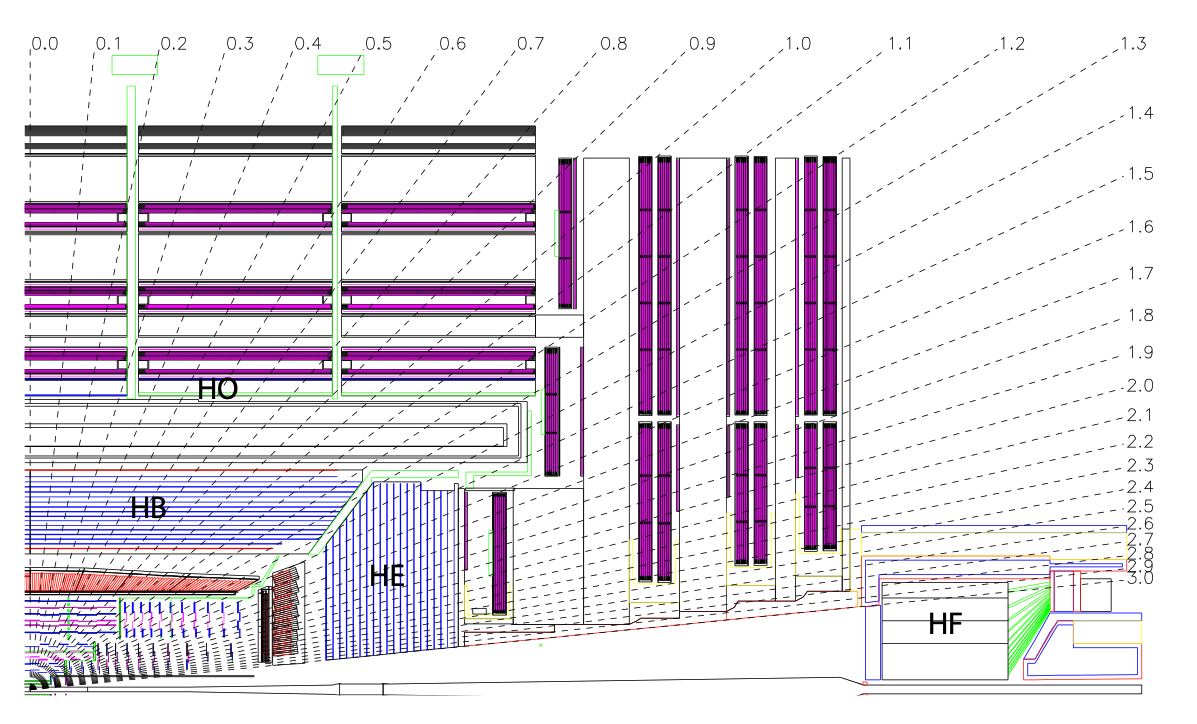
\includegraphics[width=11cm]{figures/ch-2-cern-cms/phase-1-HCAL-schematic.png}
    \caption[Longitudinal view of the CMS detector showing the hadron calorimeter barrel (HB), endcap (HE), outer (HO), and forward (HF) calorimeters.]{Longitudinal view of the CMS detector showing the hadron calorimeter barrel (HB), endcap (HE), outer (HO), and forward (HF) calorimeters from \cite{CMS-2008-JINST-3-S08004}.}
    \label{fig:phase-1-HCAL-schematic}
\end{figure}

The HB is a sampling calorimeter covering the pseudorapidity range $|\eta| < 1.3$ \cite{CMS-2008-JINST-3-S08004}. It consists of 36 identical azimuthal wedges which form two half-barrels (HB+ and HB-), with a segmentation of $(\Delta \eta, \Delta \phi) = (0.087, 0.087)$. The HE covers pseudorapidity $1.3 < |\eta| < 3$. The HB and endcap HE calorimeters are sampling calorimeters which use brass as the absorber and plastic scintillator as the active material. Light from the plastic scintillator is wavelength-shifted and captured in optic fibers which are read out by front-end electronics \cite{CMS-TDR-010-2012}. 

In the central pseudorapidity region, the combined stopping power of EB plus the HB is insufficient to contain hadron showers \cite{CMS-2008-JINST-3-S08004}. To ensure adequate sampling depth, the hadron calorimeter is extended with a tail catcher, the HO. The size and position of the tiles are designed to roughly map the layers of the HB to make towers with the same granularity of $0.087 \times 0.087$ in $\eta$ and $\phi$. HO uses the same active material as the HB and HE calorimeters, but uses the steel return yoke and magnet material of CMS as absorbers \cite{CMS-TDR-010-2012}. 


The HF is a Cherenkov calorimeter based on a steel absorber and quartz fibers which run longitudinally through the absorber and collect Cherenkov light, primarily from the electromagnetic component of showers developed in the calorimeter \cite{CMS-TDR-010-2012}. Photomultiplier tubes are used to  collect light from the quartz fibers. The HF is designed to survive in the harsh radiation conditions and high particle flux of the forward region. On average, 760\GeV per proton-proton interaction is deposited into the two forward calorimeters, compared to only 100\GeV for the rest of the detector \cite{CMS-2008-JINST-3-S08004}. Furthermore, this energy has a pronounced maximum at the highest rapidities.

\subsection{Muon detectors}
The CMS muon system is designed to have the capability of reconstructing the momentum and charge of muons over the kinematic range of the LHC, since muons are a powerful handle on signatures of interesting processes over the high background rate of the LHC \cite{CMS-2008-JINST-3-S08004}. For instance, the decay of the Standard Model Higgs boson into $ZZ$, which in turn decay to 4 leptons, can be reconstructed with high 4-particle mass resolution if all the leptons are muons, since muons are less affected than electrons by radiative losses in the tracker material. 

The muon system consists of a cylindrical barrel section and two planar endcap regions \cite{CMS-2008-JINST-3-S08004}. The barrel muon detector consists of drift tube (DT) chambers covering the pseudorapidity region $|\eta| < 1.2$ (Fig. \ref{fig:phase-1-muon-barrel-DT-schematic}). The DTs can be used as tracking detectors due to the barrel region's characteristic low neutron-induced backgrounds, low muon rate, and relatively uniform 4T magnetic field contained in the steel yoke. 

\begin{figure}[ht]
    \centering
    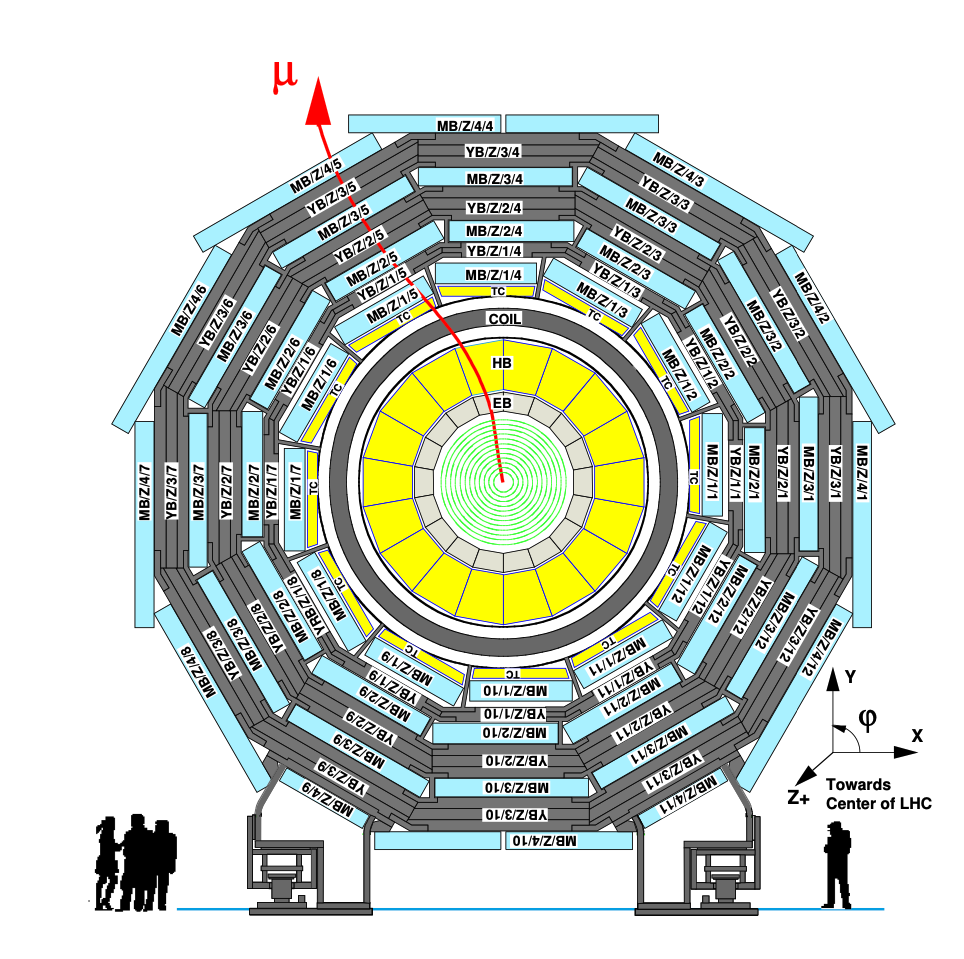
\includegraphics[width=11cm]{figures/ch-2-cern-cms/phase-1-muon-barrel-DT-schematic.png}
    \caption[Layout of the CMS barrel muon drift tube (DT) chambers in one of the five wheels.]{Layout of the CMS barrel muon drift tube (DT) chambers in one of the five wheels from \cite{CMS-2008-JINST-3-S08004}. The DTs are organized in 12 sectors of the yoke barrel (YB). In each of the 12 sectors of the yoke, there are 4 muon chambers per wheel (MB1, MB2, MB3, and MB4).}
    \label{fig:phase-1-muon-barrel-DT-schematic}
\end{figure}

In the two endcap regions, the muon rates and background levels are high and the magnetic field is large and non-uniform \cite{CMS-2008-JINST-3-S08004}. Here, the muon system uses cathode strip chambers (CSCs) to identify muons between $0.9 < |\eta| < 2.4$. The cathode strips of each chamber run radially outwards and provide a precision measurement in the $r-\phi$ bending plane. The anode wires run approximately perpendicular to the strips and are read out in order to measure $\eta$ and the beam-crossing time of a muon. 

% 2008 JINST 3 S08004, page 164
In addition to the DT and CSC, a dedicated trigger system consisting of resistive plate chambers (RPCs) in the barrel and endcap regions provide a fast, independent, and highly-segmented trigger with a sharp $p_T$ threshold over a large portion of the pseudorapidity range ($|\eta| < 1.6$) of the muon system \cite{CMS-2008-JINST-3-S08004}. RPCs have good time resolution but coarser position resolution compared to the DTs or CSCs. The RPCs also play a role in resolving ambiguities in reconstructing tracks from multiple hits in a chamber. 

\subsection{The Level-1 Trigger}
\label{section:phase-1-l1-trigger}
The design performance of the LHC corresponds to an instantaneous luminosity of $10^{34}$ cm$^{-2}$ s$^{-1}$ with a 25 ns bunch crossing rate, giving an average pile-up (number of simultaneous events) of 25 per bunch crossing \cite{CMS-TDR-012}. The large number of minimum bias events per bunch crossing, combined with the small cross-sections of possible physics discovery signatures, necessitates a sophisticated event selection system for filtering this large event rate, as it is impossible to save all events. This data filtering system is implemented by CMS in two stages. The first stage is the Level-1 (L1) Trigger, which is deployed in custom electronic hardware systems and is responsible for reducing the event rate to around 100 kHz. The second stage is the High-Level Trigger (HLT) which is described in Section \ref{section:phase-1-high-level-trigger}. This section describes the Phase-1 configuration of the Level-1 Trigger.


The L1 Trigger data flow of Phase-1 is shown in Fig. \ref{fig:phase-1-level-1-trigger-dataflow} \cite{CMS-TDR-012}, with organization into the L1 calorimeter trigger, the L1 muon trigger, and the L1 global trigger. 

\begin{figure}[ht]
    \centering
    \includegraphics[width=11cm]{figures/ch-2-cern-cms/phase-1-level-1-trigger-dataflow.png}
    \caption[Dataflow for the Phase-1 Level-1 Trigger.]{Dataflow for the Phase-1 Level-1 Trigger \cite{CMS-TDR-012}, which is implemented in custom hardware and is responsible for reducing the event rate from the LHC bunch crossing frequency of 400 MHz (bunch crossings every 25 ns) to a maximum rate of 100 kHz. In Phase-1, the Level-1 Trigger has access to information from the calorimeter and muon detectors.}
    \label{fig:phase-1-level-1-trigger-dataflow}
\end{figure}

The L1 calorimeter trigger begins with trigger tower energy sums formed by the ECAL, HCAL, and HF Trigger Primitive Generator (TPG) circuits from the individual calorimeter cell energies. In the original configuration, the ECAL energies were accompanied by a bit indicating the transverse extent of the electromagnetic energy deposits, and the HCAL energies were accompanied by a bit indicating the presence of minimum ionizing energy \cite{CERN-LHCC-2000-038}. Between Long Shutdowns 1 and 2 (LS1 and LS2), HF was upgraded to provide finer granularity information to the trigger, and the HCAL barrel and endcap front-end electronics were upgraded to provide high-precision timing information and depth segmentation information. 

In the original design of the L1 calorimeter trigger, the trigger primitives are processed by the Regional Calorimeter Trigger (RCT, upgraded to Calo Layer 1 after LS2) which finds isolated and non-isolated electron/photon candidates \cite{CMS-TDR-012}. At this stage, electrons/photons candidates are treated together since they cannot be definitively distinguished at this stage due to lack of tracking information in the L1 trigger. The Global Calorimeter Trigger (GCT, upgraded to Calo Layer 2 after LS2) sorts further the candidate electrons/photons, finds jets (classified as central, forward, and tau) using the $E_T$ sums and performs calibration of the clustered jet energies, and calculates global quantities such as missing $E_T$. It sends the top four candidates of each type to the global trigger (GT) \cite{CMS-TDR-012}.

Each of the L1 muon triggers has its own trigger logic \cite{CERN-LHCC-2000-038}. The RPC strips are connected to a Pattern Comparator Trigger (PACT), which forms trigger segments that are used to build tracks and calculate $p_{T}$. The RPC logic also provides some hit data to the CSC trigger system to resolve ambiguities caused by two muons in the same CSC. The CSCs form local charged tracks (LCTs) from the cathode strips, which are combined with the anode wire information. LCTs are combined into full muon tracks and assigned $p_{T}$ values. 

The Global Muon Trigger (GMT) sorts the RPC, DT, and CSC muon tracks, converts these tracks to the same $\eta$, $\phi$, and $p_{T}$ scale, and validates the muon sign \cite{CERN-LHCC-2000-038}. It improves the trigger efficiency by merging muon candidates that were detected in two complementary sub-systems (i.e. DT+RPC, or CSC+RPC). The GMT also contains logic to correlate the found muon tracks with an $\eta-\phi$ grid of quiet calorimeter towers to determine if the muons are isolated, as well as logic to remove duplicate candidates originating in the overlap regions from both DT and CSC systems. The final collection of muons are sorted based on their initial quality, correlation, and $p_{T}$, and the top four muons are sent to the Global Trigger \cite{CERN-LHCC-2000-038}. 

Information from the GCT and GT are sent to the Global Trigger (GT), which makes the Level-1 Accept (L1A) decision to either discard or accept the bunch crossing \cite{CERN-LHCC-2000-038}. This is accomplished by sorting ranked trigger objects that are accompanied by positional information in $\eta$ and $\phi$, permitting the trigger to applying criteria with thresholds that can vary based on the location of the trigger objects, and/or to require trigger objects to be close to or opposite from each other. The GT L1A decision arrives at the detector front end with a 3.8 $\mu$s latency after the interaction at a rate which is required to be less than 100 kHz, and triggers a full readout of the detector for further processing.



\subsection{The High-Level Trigger}
\label{section:phase-1-high-level-trigger}
The HLT is implemented in software running on a large computer farm of fast commercial processors \cite{CMS-TDR-022-HLT} \cite{Foudas:2008dt}. The algorithms in HLT have access to full data from all CMS sub-detectors, including the tracker, with full granularity and resolution. The HLT reconstruction software is similar to what is used offline for full CMS data analysis. As a result, the HLT can calculate quantities with a resolution comparable to the final detector resolution, compared to the L1 Trigger. The HLT performs more computationally-intensive algorithms, such as combining tau-jet candidates in the calorimeter with high-$p_T$ stubs in the tracker, to form a hadronic tau trigger. The maximum HLT input rate from the L1 Trigger is 100 kHz, and the HLT output rate is approximately 100 Hz. 

The HLT contains trigger paths, each corresponding to a dedicated trigger \cite{twiki_SoftwareGuide_HLT}.  A path consists of several steps implemented as software modules. Each HLT trigger path must be seeded by one or more L1 trigger bits: the first module always looks for a L1 seed, consisting of L1 bit(s) and L1 object(s). Each module performs a well-defined task such as unpacking (raw to digitized quantities), reconstruction of physics objects (electrons, muons, jet, missing transverse energy, etc.), making intermediate decisions that trigger more detailed reconstruction modules, and calculating the final decision for the trigger path. If an intermediate filter decision is negative, the rest of the path is not executed, and the trigger rejects the event.


\subsection{Particle reconstruction}
To build a description of the physics objects present in the particle collision, the basic elements from the detector layers (tracks and clusters of energy) are correlated to identify each particle in the final state. Measurements from different sub-detectors are combined to reconstruct the particle properties. This approach is called particle-flow (PF) reconstruction \cite{CERN-EP-2017-110}. Key to the success of the PF reconstruction is the fine spatial granularity of the detector layers. Coarse-grained detectors can cause the signals from different particles to merge, especially within jets. However, if the subdetectors are sufficiently segmented to separate individual particles, it becomes possible to produce a global event description that identifies all physics objects with high efficiencies and resolution.

\subsection{Data storage and computational infrastructure}

The LHC generates over 15 petabytes (15 million gigabytes) of data every year, necessitating a flexible computing system that can be accessed by researchers working at the four main LHC experiments: ALICE, ATLAS, CMS, and LHCb. The Worldwide LHC Computing Grid (WLCG) \cite{computing-Worldwide:1997398} is a global collaboration of computer centers that links thousands of computers and storage systems in over 170 centers across 41 countries. These centers are arranged in ``tiers'', and provide near real-time access to users processing, analyzing, and storing LHC data. One of the final stages of data analysis at LHC experiments is large-scale data processing taking place over distributing computing, for instance, with the use of Condor \cite{condor-article}, a distributed, scalable, flexible batch processing system which accepts a computing job, allocates a resource to it, executes it, and returns the result back to a user transparently. 
 


\chapter{The CMS Phase-1 Level-1 Trigger}

\section{The Phase-1 Level-1 Trigger}
\label{section:phase-1-l1-trigger}
The design performance of the LHC corresponds to an instantaneous luminosity of $10^{34}$ cm$^{-2}$ s$^{-1}$ with a 25 ns bunch crossing rate, giving an average pile-up (number of simultaneous events) of 25 per bunch crossing \cite{CMS-TDR-012}. The large number of minimum bias events per bunch crossing, combined with the small cross-sections of possible physics discovery signatures, necessitates a sophisticated event selection system for filtering this large event rate, as it is impossible to save all events. This data filtering system is implemented by CMS in two stages. The first stage is the Level-1 (L1) Trigger, which is deployed in custom electronic hardware systems and is responsible for reducing the event rate to around 100 kHz. The second stage is the High-Level Trigger (HLT) which is described in Section \ref{section:phase-1-high-level-trigger}. This section describes the Phase-1 configuration of the Level-1 Trigger.


The L1 Trigger data flow of Phase-1 is shown in Fig. \ref{fig:phase-1-level-1-trigger-dataflow} \cite{CMS-TDR-012}, with organization into the L1 calorimeter trigger, the L1 muon trigger, and the L1 global trigger. 

\begin{figure}[ht]
    \centering
    \includegraphics[width=11cm]{figures/ch-3-phase1-l1-trigger/phase-1-level-1-trigger-dataflow.png}
    \caption[Dataflow for the Phase-1 Level-1 Trigger.]{Dataflow for the Phase-1 Level-1 Trigger \cite{CMS-TDR-012}, which is implemented in custom hardware and is responsible for reducing the event rate from the LHC bunch crossing frequency of 400 MHz (bunch crossings every 25 ns) to a maximum rate of 100 kHz. In Phase-1, the Level-1 Trigger has access to information from the calorimeter and muon detectors.}
    \label{fig:phase-1-level-1-trigger-dataflow}
\end{figure}

The L1 calorimeter trigger begins with trigger tower energy sums formed by the ECAL, HCAL, and HF Trigger Primitive Generator (TPG) circuits from the individual calorimeter cell energies. In the original configuration, the ECAL energies were accompanied by a bit indicating the transverse extent of the electromagnetic energy deposits, and the HCAL energies were accompanied by a bit indicating the presence of minimum ionizing energy \cite{CERN-LHCC-2000-038}. Between Long Shutdowns 1 and 2 (LS1 and LS2), HF was upgraded to provide finer granularity information to the trigger, and the HCAL barrel and endcap front-end electronics were upgraded to provide high-precision timing information and depth segmentation information. 

In the original design of the L1 calorimeter trigger, the trigger primitives are processed by the Regional Calorimeter Trigger (RCT, upgraded to Calo Layer 1 after LS2) which finds isolated and non-isolated electron/photon candidates \cite{CMS-TDR-012}. At this stage, electrons/photons candidates are treated together since they cannot be definitively distinguished at this stage due to lack of tracking information in the L1 trigger. The Global Calorimeter Trigger (GCT, upgraded to Calo Layer 2 after LS2) sorts further the candidate electrons/photons, finds jets (classified as central, forward, and tau) using the $E_T$ sums and performs calibration of the clustered jet energies, and calculates global quantities such as missing $E_T$. It sends the top four candidates of each type to the global trigger (GT) \cite{CMS-TDR-012}.

Each of the L1 muon triggers has its own trigger logic \cite{CERN-LHCC-2000-038}. The RPC strips are connected to a Pattern Comparator Trigger (PACT), which forms trigger segments that are used to build tracks and calculate $p_{T}$. The RPC logic also provides some hit data to the CSC trigger system to resolve ambiguities caused by two muons in the same CSC. The CSCs form local charged tracks (LCTs) from the cathode strips, which are combined with the anode wire information. LCTs are combined into full muon tracks and assigned $p_{T}$ values. 

The Global Muon Trigger (GMT) sorts the RPC, DT, and CSC muon tracks, converts these tracks to the same $\eta$, $\phi$, and $p_{T}$ scale, and validates the muon sign \cite{CERN-LHCC-2000-038}. It improves the trigger efficiency by merging muon candidates that were detected in two complementary sub-systems (i.e. DT+RPC, or CSC+RPC). The GMT also contains logic to correlate the found muon tracks with an $\eta-\phi$ grid of quiet calorimeter towers to determine if the muons are isolated, as well as logic to remove duplicate candidates originating in the overlap regions from both DT and CSC systems. The final collection of muons are sorted based on their initial quality, correlation, and $p_{T}$, and the top four muons are sent to the Global Trigger \cite{CERN-LHCC-2000-038}. 

Information from the GCT and GT are sent to the Global Trigger (GT), which makes the Level-1 Accept (L1A) decision to either discard or accept the bunch crossing \cite{CERN-LHCC-2000-038}. This is accomplished by sorting ranked trigger objects that are accompanied by positional information in $\eta$ and $\phi$, permitting the trigger to applying criteria with thresholds that can vary based on the location of the trigger objects, and/or to require trigger objects to be close to or opposite from each other. The GT L1A decision arrives at the detector front end with a 3.8 $\mu$s latency after the interaction at a rate which is required to be less than 100 kHz, and triggers a full readout of the detector for further processing.



\chapter{The Phase-2 Upgrade of CMS}
\section{High-Luminosity LHC and CMS}
In order to sustain and extend the LHC's physics discovery program and maintain operability for a decade or more, the LHC is undergoing a major upgrade to the  High-Luminosity LHC (HL-LHC). In its final configuration, the HL-LHC will deliver a peak luminosity of $7.5 \times 10^{34}$ cm$^{-2}$ s$^{-1}$, potentially leading to total integrated luminosity of 4000 fb$^{-1}$ after ten years of operations, scheduled to begin in 2027 \cite{CMS-TDR-021}. This integrated luminosity is about ten times the predicted luminosity reach of the LHC in its initial configuration. To maximize the discovery potential of this unprecedented amount of data, the CMS detector is undergoing Phase-2 upgrades in order to perform high-precision measurements and searches for physics beyond the Standard Model in the intense running conditions of the HL-LHC.

\section{The Phase-2 Level-1 Trigger}
To achieve the goals of the HL-LHC program and to ensure the collection of information-rich datasets in the HL-LHC, the Phase-2 upgrade of the CMS Level-1 Trigger \cite{CMS-TDR-021} must be upgraded in conjunction with the CMS sub-detectors and their readouts, to maintain physics selectivity. The HL-LHC will produce an intense hadronic environment corresponding to 200 simultaneous collisions per beam crossing, necessitating comprehensive upgrades of the trigger system outlined below.

To profit from the extended coverage and increased granularity of the upgraded CMS detector, the latency of the L1 trigger system (time available to produce a L1 Accept signal) will be increased significantly from 3.8 $\mu$s to 12.5 $\mu$s, with an increased maximum output bandwidth of 750 kHz \cite{CMS-TDR-021}. With the increased latency, in addition to information from calorimeters and muon detectors (as in the Phase-1 system), information from the new tracker and high-granularity endcap calorimeter can also be included at L1 for the first time. This is illustrated in the functional diagram of the architecture of the Phase-2 trigger system in Fig. \ref{fig:phase-2-l1-architecture}. 

\begin{figure}[ht]
    \centering
    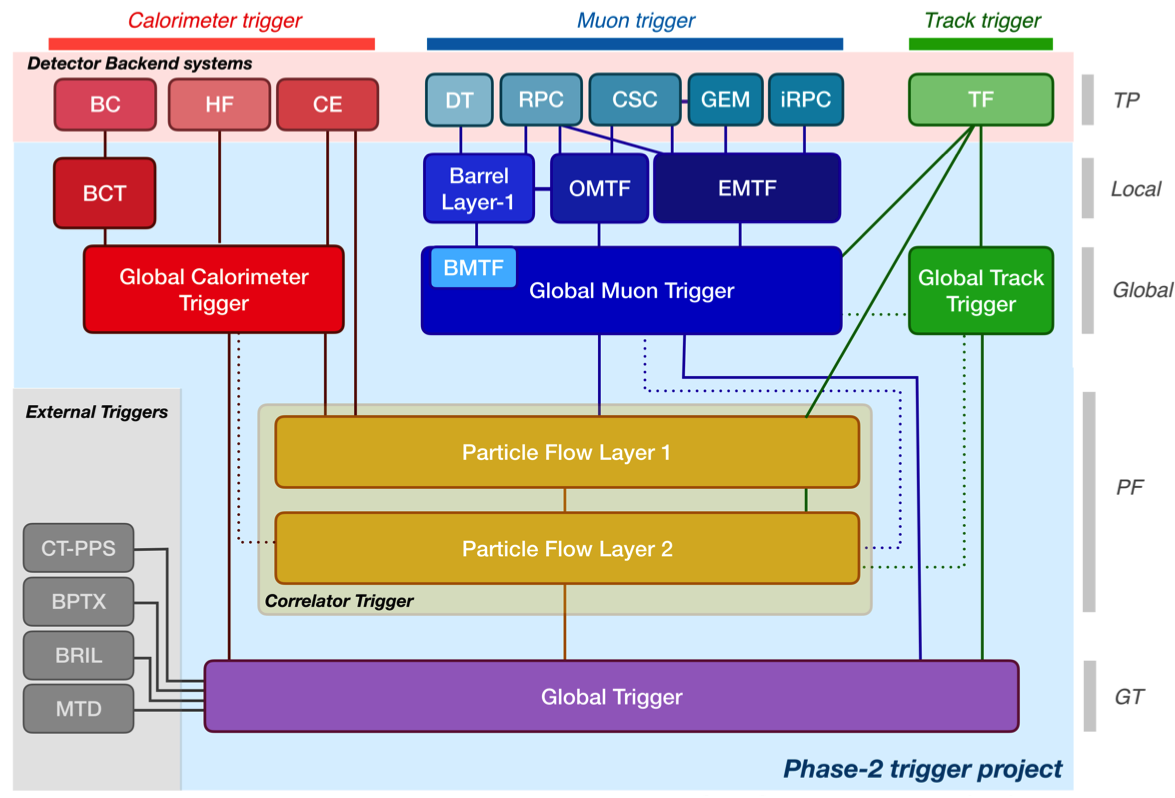
\includegraphics[width=15cm]{figures/ch-4-phase2/phase-2-l1-architecture.png}
    \caption[Functional diagram of the CMS L1 Phase-2 upgraded trigger design.]{Functional diagram of the CMS L1 Phase-2 upgraded trigger design \cite{CMS-TDR-021}, showing the four trigger paths: calorimeter, muon, track, and Particle Flow. For the first time, tracking information will be available as early as the L1 Trigger.}
    \label{fig:phase-2-l1-architecture}
\end{figure}

The key feature of the Phase-2 L1 Trigger is the introduction of a correlator layer, where algorithms produce higher-level trigger objects by combining information from sub-detectors, with a selectivity approaching that of offline reconstruction in the HLT \cite{CMS-TDR-021}. Four independent data processing paths (grouped together in Fig. \ref{fig:phase-2-l1-architecture}) are implemented: tracking, calorimetry, muon systems, and particle-flow techniques:
\begin{itemize}
    \item \textbf{Calorimeter Trigger path:} (\textit{red}, Fig. \ref{fig:phase-2-l1-architecture}) A barrel calorimeter trigger (BCT) and the HGCAL backend are used to produce high-granularity information from the calorimeters to produce high-resolution clusters and identification variables used for later processing. Outputs from the BCT, HGCAL, and the HF are sent to a global calorimeter trigger (GCT), where calorimeter-only objects such as $e/\gamma$ candidates, hadronically decaying tau lepton candidates, jets, and energy sums are built.
    \item \textbf{Track Trigger path:} (\textit{green}, Fig. \ref{fig:phase-2-l1-architecture}) Tracks from the Outer Tracker are reconstructed in the track finder (TF) processors as part of the detector backend. A global track trigger (GTT) will reconstruct the primary vertices of the event, along with tracker-only based objects, such as jets and missing transverse momentum.
    \item \textbf{Muon Trigger path:} (\textit{blue}, Fig. \ref{fig:phase-2-l1-architecture}) Trigger primitives are processed by muon track finder algorithms, again separated into the barrel (barrel muon track finder, BMTF), overlap (overlap muon track finder, OMTF), and endcap (endcap muon track finder, EMTF). Standalone muons and stubs containing information such as position, bend angle, and timing, as well as L1 tracks, are sent to the global muon trigger (GMT).
    \item \textbf{Particle-Flow Trigger path:} (\textit{yellow}, Fig. \ref{fig:phase-2-l1-architecture}) The correlator trigger (CT) aims to approach the performance of offline Particle Flow, and is implemented in two layers. ``Layer-1'' produces the particle-flow candidates from matching calorimeter clusters and tracks. ``Layer 2'' builds and sorts final trigger objects and applies additional identification and isolation criteria.
\end{itemize}

The outputs from the above trigger paths are combined in the Global Trigger (GT) (\textit{purple}, Fig. \ref{fig:phase-2-l1-architecture}), which calculates the final trigger decision (Level-1 Accept), transmitting it to the Trigger Control and Distribution System (TCDS), which distributes it to the detector backend systems, initiating the readout to the DAQ. The GT also provides the interface to external triggers (\textit{grey}, Fig. \ref{fig:phase-2-l1-architecture}), such as triggers for the precision proton spectrometer (PPS), beam position and timing monitors (BPTX), and luminosity and beam monitoring (BRIL) detectors \cite{CMS-TDR-021}. The design of the Phase-2 Level-1 Trigger allows for future inclusion of triggering information, for instance information about minimum ionizing particles (MIPs) from the MIP Timing Detector (MTD) \cite{CERN-LHCC-2017-027}.

\section{Standalone Barrel Calorimeter electron/photon reconstruction}
\begin{figure}[ht]
    \centering
    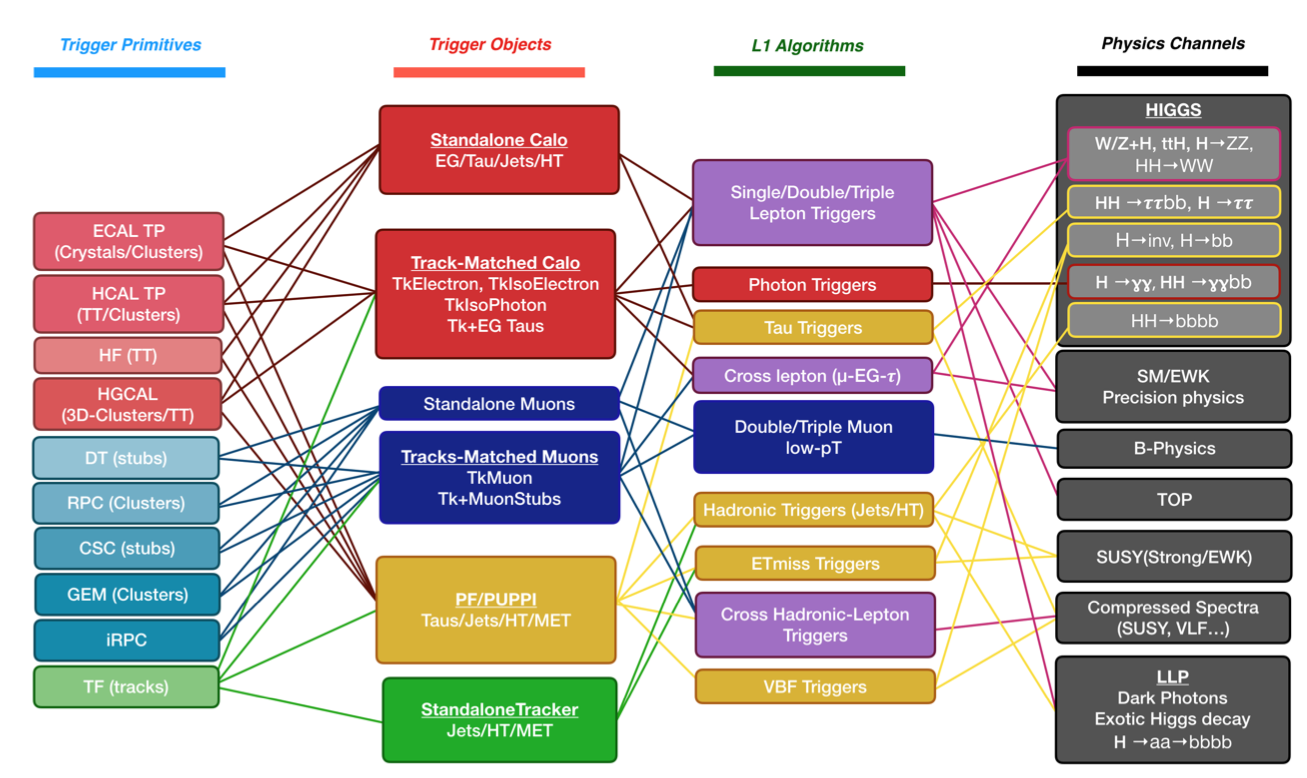
\includegraphics[width=15cm]{figures/ch-4-phase2/phase-2-summary-trigger-TP-algo-physics.png}
    \caption[Summary of the links between the trigger primitives, the trigger objects, the Level-1 algorithms, and the physics channels in the Phase-2 menu.]{Summary of the links between the trigger primitives (\textit{first column}), the trigger objects (\textit{second column}), the Level-1 algorithms used in the menu (\textit{3rd column}), and the physics channels (\textit{4th column}), from \cite{CMS-TDR-021}, where a full description of the Phase-2 L1 algorithms can be found. This work focuses on developments for the Standalone Calorimeter electron and photon ("EG") reconstruction algorithm.}
    \label{fig:phase-2-summary-trigger-TP-algo-physics}
\end{figure}

The reconstruction and identification of electrons and photons ($e/\gamma$) begin with the trigger primitives of the barrel ECAL and HCAL detectors and endcap HGCAL calorimeters, covering the pseudorapidity region $|\eta| < 3$. The barrel and endcap regions of the detector are intrinsically different enough to warrant different approaches to $e/\gamma$ reconstruction. This work focuses on the Standalone Calorimeter $e/\gamma$ reconstruction taking place in the barrel (Fig. \ref{fig:phase-2-summary-trigger-TP-algo-physics}).

\subsection{Phase-2 geometry of the ECAL Barrel trigger}
\label{section:phase-2-ECAL-barrel-geometry}
% https://cds.cern.ch/record/2714892/files/CMS-TDR-021.pdf  
% Section 2.2.1, on page 36-37
In Phase-2, the upgrade of both on-detector and off-detector electronics for the barrel calorimeters trigger primitive generator (TPG) will stream single crystal data from the on-detector to the backend electronics, in contrast to the lower-granularity output of the Phase-1 ECAL TPG that is restricted to providing trigger tower sums of $5 \times 5$ crystals \cite{CMS-TDR-021}. 
A schematic representation of the geometry of the ECAL barrel in the Regional Calorimeter Trigger (RCT) is shown in Fig. \ref{fig:phase-2-rct-cards-schematic}. The barrel is spanned by 36 RCT cards, each spanning $17 \times 4$ towers in $\eta \times \phi$. Each RCT card is subdivided into five ``regions'' as shown in Fig. \ref{fig:phase-2-one-rct-card-schematic}. After initial clustering and processing, the outputs of the RCT card are sent to the Global Calorimeter (GCT) trigger, which is processed in three cards as shown in Fig. \ref{fig:phase-2-gct-cards-schematic}.

\begin{figure}[ht]
    \centering
    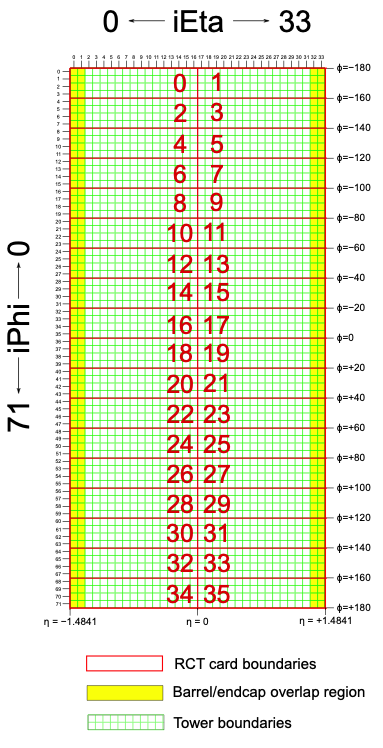
\includegraphics[width=9cm]{figures/ch-4-phase2/phase-2-rct-cards-schematic.png}
    \caption{Schematic of the geometry of the Phase-2 ECAL barrel in the Regional Calorimeter Trigger (RCT), showing the division of the barrel region into 36 Regional Calorimeter Trigger (RCT) cards (\textit{red}). Each card spans $17 \times 4$ towers in $\eta \times \phi$ (\textit{green}), and each tower is $5\times 5$ in single crystals in $\eta \times \phi$. Towers in the overlap region (\textit{shaded yellow}) are read out to both the barrel and endcap.}
    \label{fig:phase-2-rct-cards-schematic}
\end{figure}

\begin{figure}[ht]
    \centering
    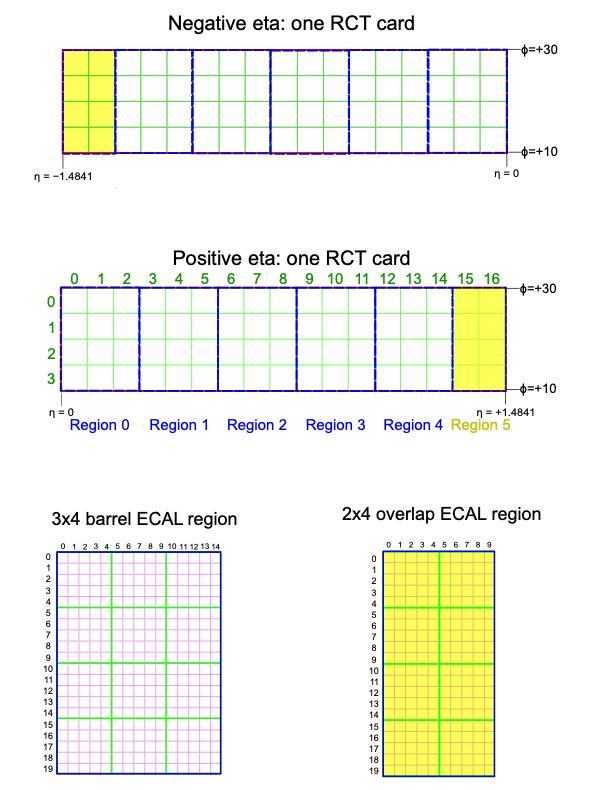
\includegraphics[width=9cm]{figures/ch-4-phase2/phase-2-one-rct-card-schematic.png}
    \caption{Schematic of two example RCT cards in the negative eta (\textit{top}) and positive eta (\textit{center}) regions of the ECAL barrel. Each RCT card is divided into five regions: four regions are of size $3 \times 4$ towers in $\eta \times \phi$ (\textit{bottom left}), and a fifth smaller overlap region of size $2 \times 4$ towers (\textit{bottom right}). Each tower is $5 \times 5$ ($\eta\times\phi$) in crystals.}
    \label{fig:phase-2-one-rct-card-schematic}
\end{figure}


\begin{figure}[ht]
    \centering
    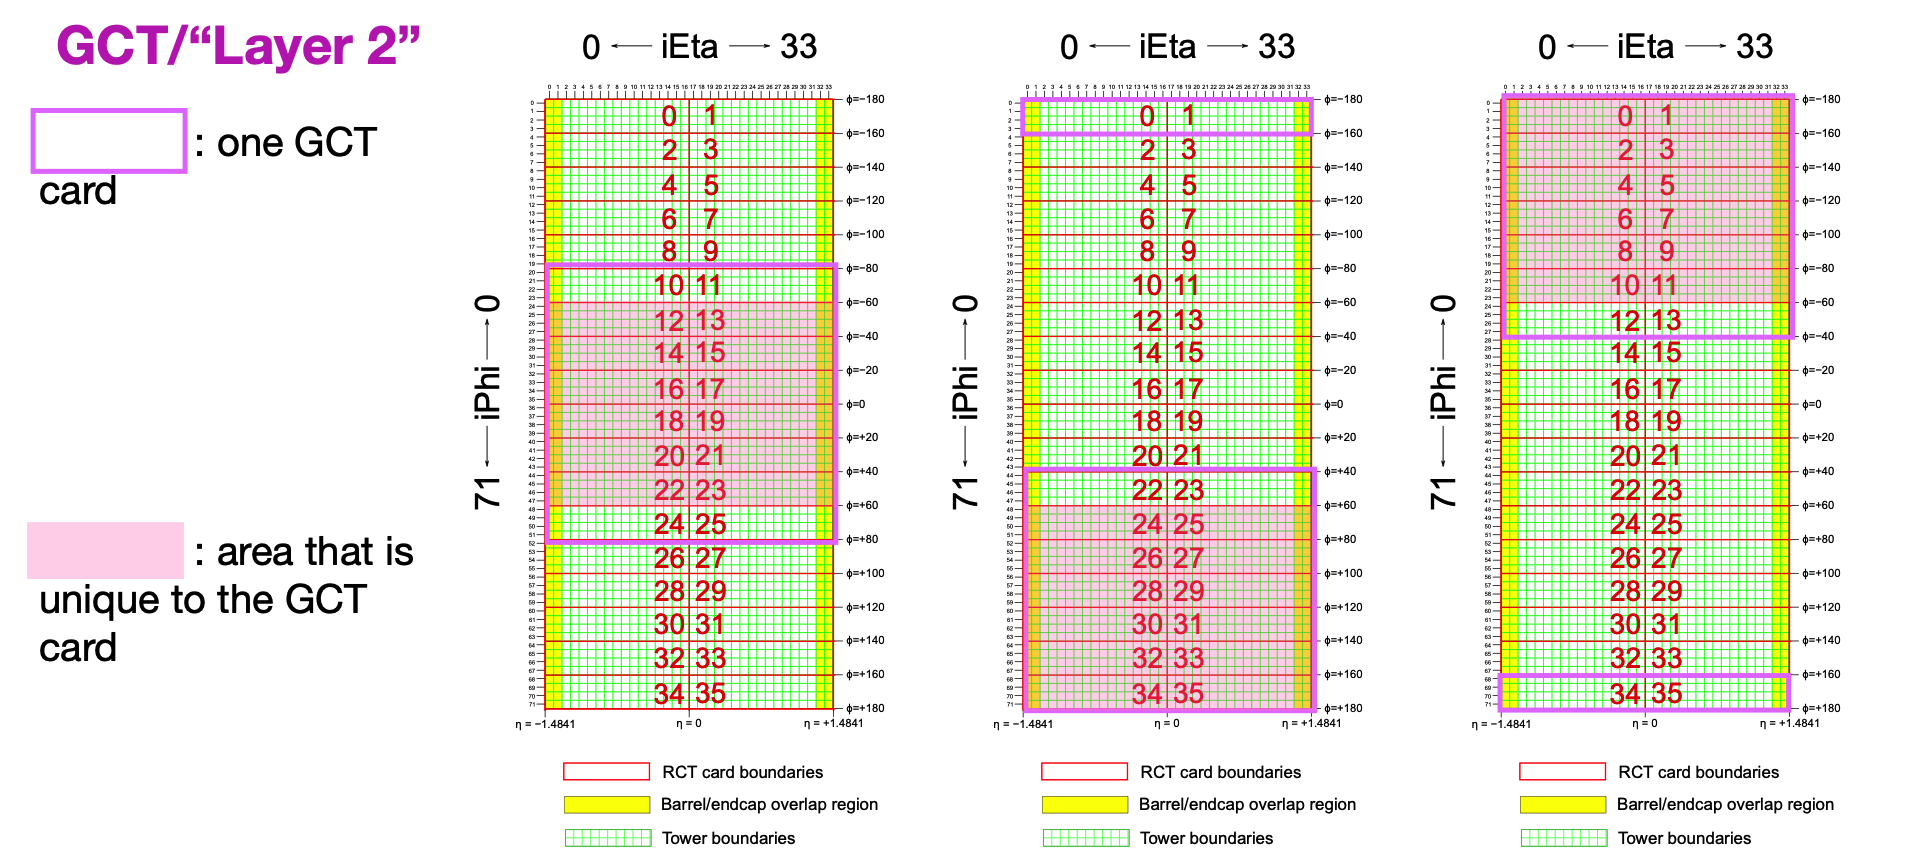
\includegraphics[width=15cm]{figures/ch-4-phase2/phase-2-gct-cards-schematic.png}
    \caption{Schematic of the Phase-2 ECAL barrel in the Global Calorimeter Trigger (GCT), which will process the outputs of the Regional Calorimeter Trigger (RCT) in three cards (\textit{magenta highlights}). Each card in the GCT processes the equivalent of sixteen RCT cards, with the center twelve being unique to that GCT card (\textit{shaded pink}), and the remaining four processed in overlap with the other GCT cards.}
    \label{fig:phase-2-gct-cards-schematic}
\end{figure}


\subsection{Phase-2 electron/photon reconstruction algorithm}
\label{section:phase-2-egamma-reconstruction-algorithm}

The standalone barrel algorithm for reconstructing and identifying electrons and photons in the Phase-2 Level-1 Trigger takes as input the digitized response of each crystal of the barrel ECAL, with a granularity $0.0175 \times 0.0175$ in $\eta \times \phi$, which is 25 times higher than the input to the Phase-1 trigger, which consisted of trigger towers with a granularity of $0.0875 \times 0.0875$. In HCAL the tower size of $0.0875 \times 0.0875$ is unchanged. The trigger algorithm is designed to closely reproduce the algorithm used in the offline reconstruction, with limitations and simplifications due to trigger latency. 

\begin{figure}[ht]
    \centering
    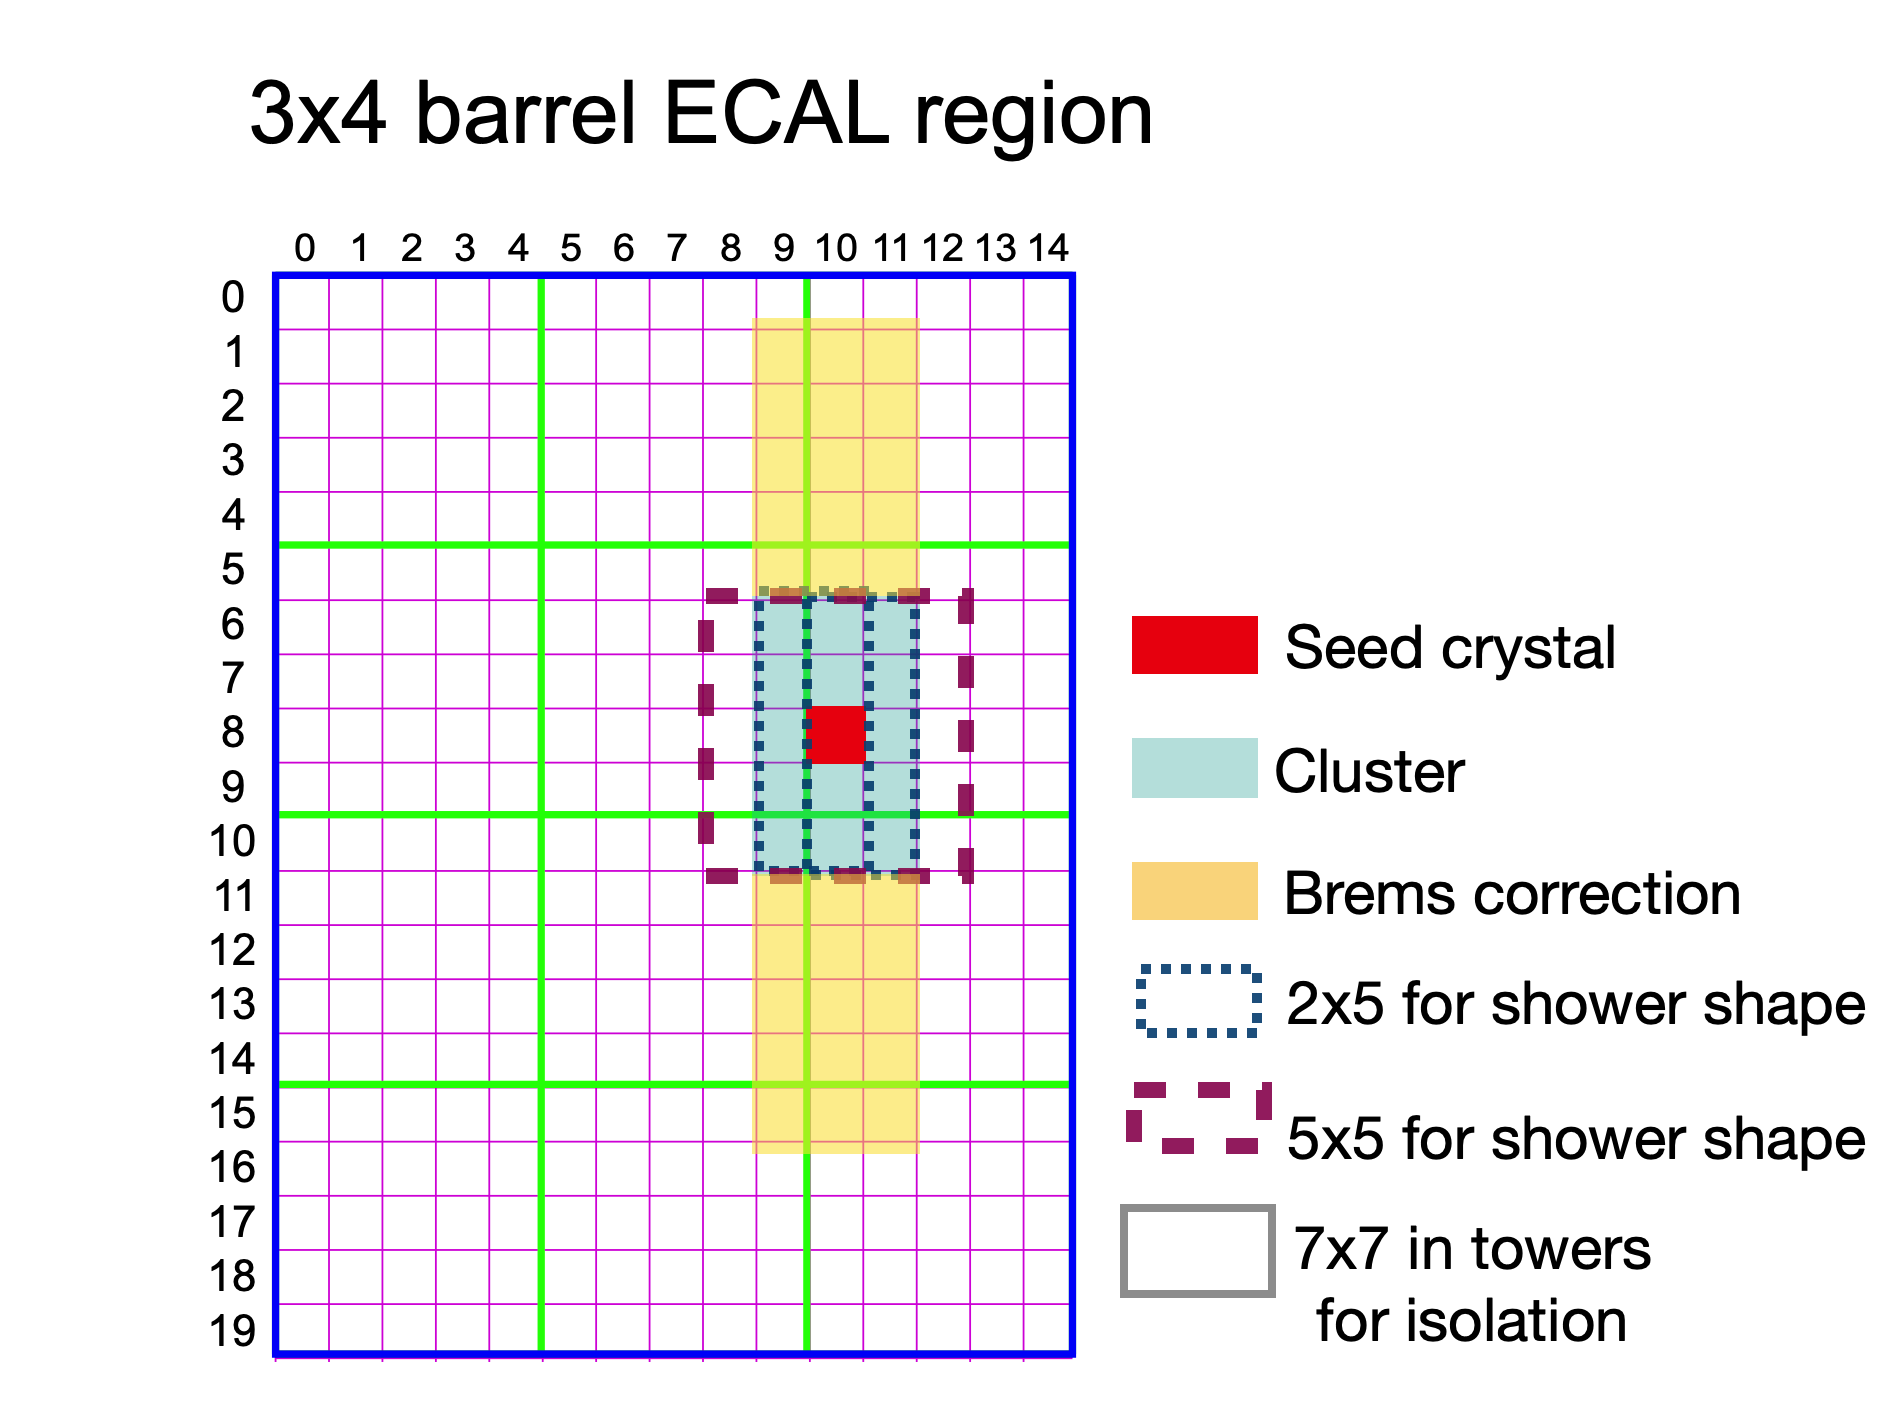
\includegraphics[width=12cm]{figures/ch-4-phase2/phase-2-cluster-footprint.png}
    \caption{Illustration of an example electron/photon ($e/\gamma$) cluster in the Phase-2 Level-1 Trigger standalone barrel $e/\gamma$ reconstruction, in a region of $15\times 20$ crystals ($3\times 4$ towers). Each small pink square is one crystal, the highest-granularity ECAL trigger primitives available to the L1 Trigger in Phase-2. The core cluster consists of the energy sum in a $3\times 5$ window of crystals, (\textit{shaded light blue}) centered around the seed crystal (\textit{red}). Bremsstrahlung corrections are checked in the adjacent $3\times 5$ windows in the $\phi$ direction (\textit{shaded light yellow}). The relative energies in windows of size $2\times 5$ and $5\times 5$ in crystals (\textit{dashed dark blue and dark red}) are used to compute shower shape variables to identify true $e/\gamma$ objects. Lastly, an isolation sum is computed in a window of size $7\times 7$ in towers (not shown in figure).}
    \label{fig:phase-2-cluster-footprint}
\end{figure}


In the RCT, an initial requirement of $p_{T} > 0.5$ GeV is imposed on the input trigger primitives (i.e. energies from the ECAL crystals and HCAL towers) to reject contribution from pileup. In one of the regions inside a RCT card (Fig. \ref{fig:phase-2-one-rct-card-schematic}), the crystal containing the highest energy deposit is identified as the seed crystal, as shown in Fig. \ref{fig:phase-2-cluster-footprint}. The energy in the crystals in a window of size $3\times 5$ in $\eta\times\phi$ around the seed cluster is added into a cluster. The energy is considered ``clustered''. The process is repeated with the remaining ``unclustered" energy, until up to four clusters are produced in the region. 


To improve $e/\gamma$ identification and to reduce background contributions, identification and reconstruction algorithms are implemented at this stage:
\begin{itemize}
    \item Shower shape: The energy deposit sums around the seed crystal is computed in windows of size $2 \times 5$ and $5 \times 5$ (Fig. \ref{fig:phase-2-cluster-footprint}, \textit{dashed lines}), with true $e/\gamma$ clusters tending to produce showers that deposit most of their energy in a $2 \times 5$ region. 
    \item Bremsstrahlung recovery: $e/\gamma$ tend to spread in the $\phi$ direction due to charged particles being bent by the magnetic field of the CMS solenoid. If sufficient energy comparable to the core $3 \times 5$ cluster is found in the adjacent $3 \times 5$ windows (Fig. \ref{fig:phase-2-cluster-footprint}, \textit{shaded yellow}), the energy is added to the core cluster and no longer considered unclustered energy.
\end{itemize}

After parallel processing in the regions, the clusters in a RCT card are stitched together if they are located directly along the borders of a region (Fig. \ref{fig:phase-2-rct-cards-schematic}). The remaining unclustered ECAL energy is summed into ECAL towers. 

From each RCT card, the twelve highest-energy clusters, as well as any remaining unclustered energy, are sent to the GCT. Since each GCT card has information from sixteen RCT cards (Fig. \ref{fig:phase-2-gct-cards-schematic}), final stitching across the boundaries of the RCT cards is performed. One more identification algorithm is performed at this stage:
\begin{itemize}
    \item Isolation: One handle to reject backgrounds from e.g. pileup, comes from the tendency for background to be spread more uniformly across a large area in the detector, whereas genuine $e/\gamma$ are expected to produce showers concentrated in the $3 \times 5$ crystal window. The energy sum in a large window of $7 \times 7$ in towers is computed and used to reject background.
\end{itemize}

\begin{figure}[ht]
    \centering
    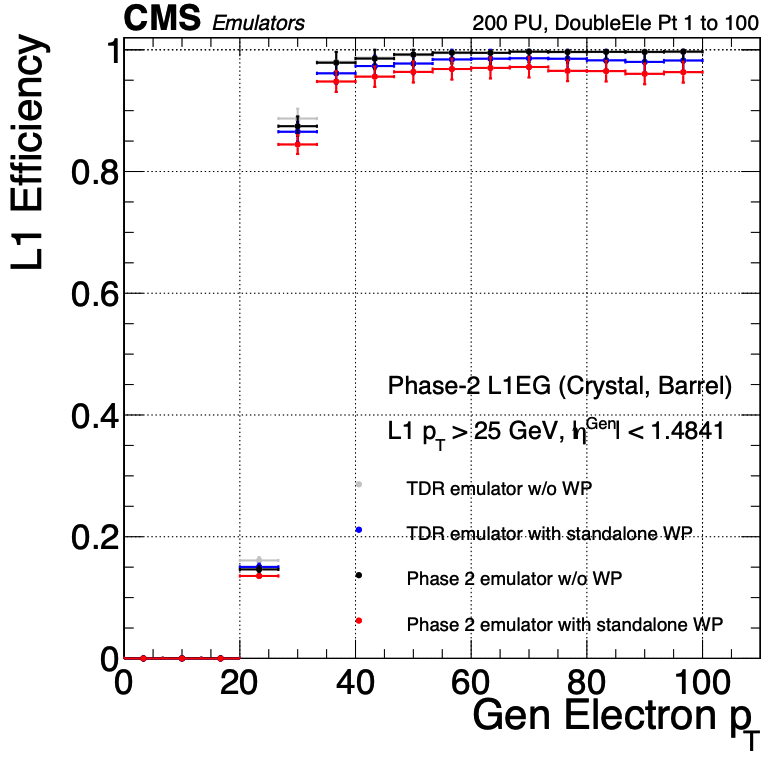
\includegraphics[width=12cm]{figures/ch-4-phase2/results-egamma-efficiency-gt25.png}
    \caption[Efficiency of the standalone barrel $e/\gamma$ reconstruction, as a function of the true electron's transverse momentum $p_{T}$.]{Efficiency of the standalone barrel $e/\gamma$ reconstruction, measured in a simulated sample of electrons, as a function of the true electron's transverse momentum $p_{T}$. The performance of the previous, idealized algorithm as shown in the 2021 Phase-2 TDR \cite{CMS-TDR-021} with and without the isolation and shower shape discrimination variables (``standalone working point/ WP'') (\textit{dark blue, grey}). The Phase-2 emulator discussed in this work with and without the same working point (\textit{black, red}) is shown to have comparable performance.}
    \label{fig:results-egamma-efficiency-gt25}
\end{figure}

\begin{figure}[ht]
    \centering
    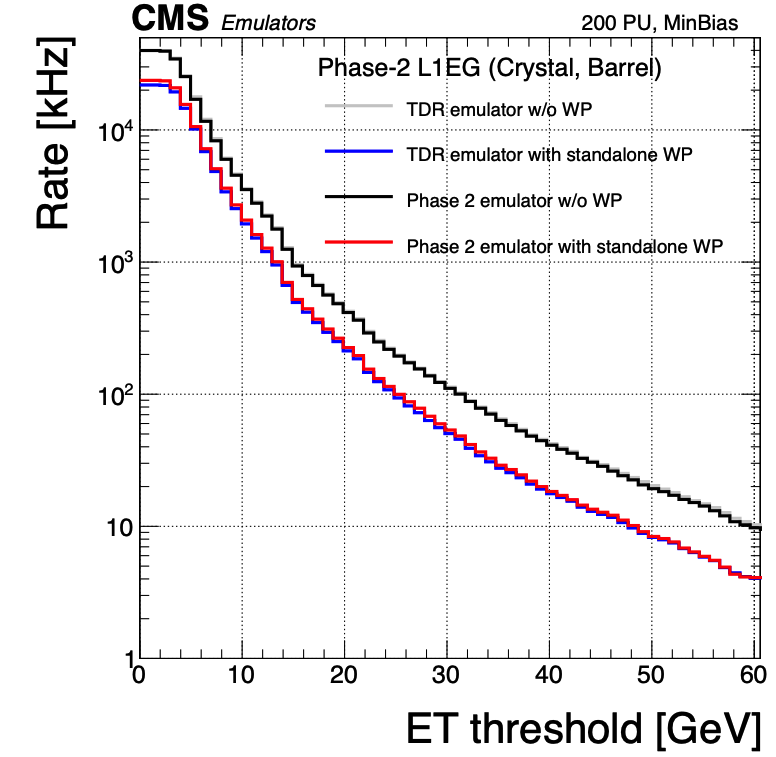
\includegraphics[width=12cm]{figures/ch-4-phase2/results-egamma-rates.png}
    \caption[Rates of the standalone barrel $e/\gamma$ reconstruction measured as a function of the minimum energy ($E_T$) required of the reconstructed $e/\gamma$ object in each event.]{Rates of the standalone barrel $e/\gamma$ reconstruction, evaluated on a minimum bias sample, measured as a function of the minimum energy ($E_T$) required of the reconstructed $e/\gamma$ object in each event. The performance of the previous, idealized algorithm as shown in the 2021 Phase-2 TDR \cite{CMS-TDR-021} with and without the isolation and shower shape discrimination variables (``standalone working point/ WP'') (\textit{dark blue, grey}). The Phase-2 emulator discussed in this work with and without the same working point (\textit{black, red}) is shown to have comparable performance.}
    \label{fig:results-egamma-rates}
\end{figure}


The performance of the standalone barrel $e/\gamma$ algorithm in Phase-2 conditions is summarized in the efficiency and rates. The efficiencies are measured with a simulated Monte Carlo sample containing electrons. The rates are measured with a simulated minimum bias sample intended to closely mimic generic proton-proton collisions in the CMS detector. The performance of the Phase-2 emulator discussed in this work, which closely mimics the firmware logic and uses fixed-precision integers, is shown to be comparable to the previous emulator which used floats and idealized logic.



\chapter{Event reconstruction}
We review the properties of the particles most pertinent to the analyes presented in this work (taus, muons, electrons, and b-jets), their resulting signatures in the CMS detector, and dedicated reconstruction techniques used at CMS.

\section{Taus}
Tau leptons, with a mass of 1.776 GeV, are heavy enough to decay hadronically (i.e. to final states with hadrons) which it does so about 64.8\% of the time. These hadronic decays are denoted $\tau_{h}$. The remainder of the time, it decays to final states with the lighter leptons (electron or muon), termed leptonic decays. In all cases, at least one is produced, resulting in missing transverse energy in the CMS detector. The tau's largest decay branching ratios (proportional to probability of decay) are listed below \citep{workman_review_2022}: 
\begin{itemize}
    \item 25.5\% decay to $\pi^- \pi^0 \nu_{\tau}$
    \item 17.8\% decay to $e^- \bar{\nu}_e \nu_{\tau}$
    \item 17.4\% decay to $\mu^- \bar{\nu}_\mu \nu_{\tau}$
    \item 10.8\% decay to $\pi^- \nu_{\tau}$ (excluding $K^0, \omega$)
    \item 9.3\% decay to $\pi^- 2\pi^0 \nu_{\tau}$ (excluding $K^0, \omega$)
    \item 9.0\% decay to $\pi^- \pi^- \pi^+ \nu_{\tau}$ (excluding $K^0, \omega$)
\end{itemize}

Thus in analyses containing $\tau\tau$ states, a distinction of the final states must be made for the possible combinatorics of the tau final states. For instance, a $\mu\tau_{h}$ event channel must be treated differently than a $\tau_{h}\tau_{h}$ channel.

In the CMS detector, charged pions leave tracks in the tracking detector before being absorbed in the hadronic calorimeter. Due to presence of the tracks for the charged pions, they are called ``prongs'' in hadronic tau reconstruction, giving gives rise to the names ``1 prong", ``1 prong + $\pi^0$(s)", and ``3-prong'' for the dominant hadronic tau decay modes. Neutral pions decay to two photons which lose their energy in the electromagnetic calorimeter. Taus that decay to electrons and muons, are typically triggered on and reconstructed as electrons and muons respectively. 

At CMS, hadronically decaying tau leptons are reconstructed with the hadron-plus-strips (HPS) algorithm \citep{CMS-TAU-14-001}, which is seeded with anti-$k_T$ jets. The HPS algorithm reconstructs $\tau_{h}$ candidates on the basis of the number of tracks and the number of ECAL strips in the $\eta-\phi$ plane with energy deposits, in the 1 prong, 1 prong + $\pi^0$(s), and 3-prong decay modes. A multivariate (MVA) discriminator, including isolation and lifetime information, is used to reduce backgrounds from quark- and gluon-initiated jets that are misidentified as $\tau_{h}$ candidates. 

\section{Muons}
Muons are identified with requirements on the quality of the track reconstruction and on the number of measurements in the tracker and the muon systems \citep{CMS-MUO-10-004}. In the standard CMS reconstruction, tracks are first reconstructed independently in the inner tracker (tracker track) and in the muon system (standalone-muon track). Next, these tracks are processed in two different methods. The first is Global Muon reconstruction (outside-in), which fits combined hits from the tracker track and standalone-muon track, using the Kalman-filter technique. At large transverse momenta, $p_{T} \gtrsim 200$ GeV, the global-muon fit can improve the momentum resolution compared to the tracker-only fit.  The second is Tracker Muon reconstruction (inside-out), which starts with tracker tracks with $p_{T} > 0.5$ GeV and total momentum $p_{T} > 2.5$ GeV. These tracks are extrapolated outwards to the muon system and matched to detector segments there, taking into account the magnetic field, expected energy losses, and multiple Coulomb scattering in the detector material. Tracker Muon reconstruction is more efficient than the Global Muon reconstruction at low momenta, $p \lesssim 5$ GeV, because it only requires a single muon segment in the muon system, where as Global Muon reconstruction typically requires segments in at least two muon stations.

\section{Electrons}
Electrons are identified with a multivariate discriminant combining several quantities describing the track quality, the shape of the energy deposits in the ECAL, and the compability of the the measurements from the tracker and the ECAL \citep{JINST-2015-10-P06005}.


\section{B-jets}






% \appendix
% \chapter{Code}
% \input{./Chapters/code}


\bibliography{Thesis} \label{bib}
%\nocite{*}

\end{document}



